\documentclass[11pt,a4paper]{article}

% ------------------------------------------------------------
% Packages
% ------------------------------------------------------------
\usepackage[margin=2.5cm]{geometry}
\usepackage{graphicx}
\usepackage{float}
\usepackage{amsmath, amssymb}
\usepackage{booktabs}
\usepackage{array}
\usepackage{xcolor}
\usepackage{hyperref}
\usepackage{listings}
\usepackage{caption}
\usepackage{subcaption}
\usepackage{enumitem}
\usepackage[utf8]{inputenc}
\usepackage[T1]{fontenc}
\usepackage{lmodern}
\usepackage{algorithm}
\usepackage{algpseudocode}
\usepackage[toc,page]{appendix}
\usepackage{upquote}

% ------------------------------------------------------------
% Hyperref setup
% ------------------------------------------------------------
\hypersetup{
    colorlinks=true,
    linkcolor=blue,
    urlcolor=blue,
    citecolor=blue
}

% ------------------------------------------------------------
% Code listing setup
% ------------------------------------------------------------
\lstset{
    basicstyle=\ttfamily\small,
    breaklines=true,
    frame=single,
    columns=fullflexible,
    keepspaces=true,
    upquote=true,
    showstringspaces=false,
    backgroundcolor=\color{gray!5},
    keywordstyle=\color{blue!70!black},
    commentstyle=\color{green!40!black},
    stringstyle=\color{orange!80!black}
}

% ------------------------------------------------------------
% Title information
% ------------------------------------------------------------
\title{
    \textbf{Movers SAT Solver: Report}\\
    \large Optimal Logistics Planning Using Boolean Satisfiability
}

\author{
    \textbf{Group:} Group C\\[0.5em]
    \textbf{Members:}\\
    Giovanni Barbieri\\
    Vasyl Damian\\
    Simona Di Lena\\
    Cristian Nicolae Gheorghe\\
    Simone Maccario\\
    Patrick Magnani\\
    Massimiliano Nicol\\[0.5em]
    \textbf{Course:} Theory of Computation
}

\date{\today}

\begin{document}

    \maketitle

    \begin{center}
        \vspace{1em}
        \textit{This report describes the design and implementation of a SAT-based solver for the movers problem.}
    \end{center}

    \newpage

    \tableofcontents

    \newpage

    \section{Introduction} \label{sec:introduction}
The goal of this project is to model and solve the \textit{movers problem} using Boolean satisfiability (SAT).
The problem consists of emptying an $n$-floor building with a team of $m$ movers.
The building contains a number of items located on different floors, and all persons and items must eventually end on the ground floor, represented as floor $0$.

\noindent Time is assumed to be discrete.
At every time step, each mover may perform one of the available actions:
\[
    \texttt{ascends}(p,t), \qquad
    \texttt{descends}(p,t), \qquad
    \texttt{carries}(p,i,t),
\]
where $p$ is a person, $i$ is an item, and $t$ is a time step.
The action \texttt{ascends} moves a person up one floor, \texttt{descends} moves a person down one floor, and \texttt{carries} represents a person carrying an item down one floor while descending.
Each action takes exactly one time step.

\noindent The project was implemented as a complete SAT-based logistics planning system.
The backend encodes the problem as a conjunctive normal form (CNF) formula and solves it using the Glucose3 SAT solver through the PySAT library.
The frontend provides an interactive graphical interface where users can configure the number of floors, movers, items, and solving mode, then visualize the computed plan step by step.

\noindent The final system supports two task variants:

\begin{itemize}
    \item \textbf{Task 1: Movement Only.} Movers start at floor $0$ and must reach specified target floors within a given time horizon.
    \item \textbf{Task 2: Movement and Carrying.} Movers and items must all end on floor $0$.
    Items can only move downward when carried by a descending mover.
\end{itemize}

\noindent The main objective of the solver is not only to check whether a plan exists for a fixed number of steps, but also to find the shortest valid plan using iterative deepening over the time horizon.
    \newpage

    \section{System Architecture} \label{sec:system-architecture}
The system is divided into two main components: a Python backend and a Vue frontend.
The backend is responsible for the formal SAT encoding, solver execution, model decoding, and output generation.
The frontend is responsible for user interaction, input validation, and visualization of the computed plan.

\begin{figure}[H]
    \centering
    \fbox{
        \begin{minipage}{0.9\textwidth}
            \centering
            User Input (Frontend or CLI)\\
            $\downarrow$\\
            Problem Configuration\\
            $\downarrow$\\
            SAT Encoder\\
            $\downarrow$\\
            CNF Formula + Variable Mapping\\
            $\downarrow$\\
            Glucose3 SAT Solver\\
            $\downarrow$\\
            Model Decoder\\
            $\downarrow$\\
            Human-Readable Plan + Visualization
        \end{minipage}
    }
    \caption{General pipeline of the Movers SAT Solver.}
    \label{fig:pipeline}
\end{figure}

\subsection{Backend Architecture} \label{subsec:backend-architecture}

The backend is implemented in Python using FastAPI\@.
It exposes REST endpoints that allow the frontend to send a problem instance and receive either a satisfiable plan or an unsatisfiable result.

\noindent The backend is organized into the following main modules:

\begin{itemize}
    \item \texttt{models/problem.py}: defines the Pydantic models for problem inputs and solver outputs.
    \item \texttt{encoding/variables.py}: defines the Boolean variable families and maps symbolic variables to integer identifiers.
    \item \texttt{encoding/common\_clauses.py}: provides reusable CNF helpers such as at-most-one, at-least-one, and exactly-one constraints.
    \item \texttt{encoding/task1\_encoder.py}: encodes the movement-only problem.
    \item \texttt{encoding/task2\_encoder.py}: extends Task 1 with item movement and carrying constraints.
    \item \texttt{solver/runner.py}: runs Glucose3 either for a fixed time horizon or with iterative deepening.
    \item \texttt{solver/decoder.py}: converts a satisfying SAT assignment into a readable sequence of time steps.
    \item \texttt{output/dimacs.py}: serializes the generated CNF formula in DIMACS format.
    \item \texttt{output/mapping.py}: exports the variable mapping as JSON\@.
    \item \texttt{api/routes.py}: defines the REST API endpoints.
\end{itemize}

\noindent The API provides endpoints for solving a problem optimally, solving at a fixed horizon, downloading the DIMACS CNF file, and downloading the variable mapping.

\subsection{Frontend Architecture} \label{subsec:frontend-architecture}

The frontend is implemented using Vue and Tailwind CSS\@.
It communicates with the backend through a small API client that sends JSON payloads to the FastAPI server and retrieves solver results.

\noindent The frontend is divided into several components:

\begin{itemize}
    \item \texttt{App.vue}: maintains the global form state and coordinates solver requests.
    \item \texttt{ProblemSetup.vue}: provides the form where the user selects the task type, number of floors, number of movers, items, and advanced solver options.
    \item \texttt{ResultsPanel.vue}: displays solver status, runtime, number of steps, playback controls, and download buttons.
    \item \texttt{BuildingVisualizer.vue}: renders the building floors and places movers and items on the correct floors for the selected time step.
    \item \texttt{ActionLog.vue}: lists the actions performed by each mover at the current time step.
\end{itemize}

\noindent The interface allows two solving modes:

\begin{itemize}
    \item \textbf{Iterative Deepening:} searches for the shortest valid solution up to a maximum number of steps.
    \item \textbf{Fixed Horizon:} checks whether a solution exists for an exact number of time steps.
\end{itemize}

\noindent When a solution is found, the user can play through the sequence using timeline controls.
The frontend allows the user to download the generated DIMACS CNF instance and the variable mapping.
The satisfying model returned by the SAT solver is decoded into the displayed step-by-step plan.

    \newpage

    \section{Theoretical Background} \label{sec:theoretical-background}
Boolean satisfiability is the problem of determining whether there exists an assignment of truth values to Boolean variables that makes a propositional formula true.
A formula in conjunctive normal form (CNF) is a conjunction of clauses, where each clause is a disjunction of literals.

\noindent The movers problem is naturally modeled as a planning problem over discrete time.
Instead of searching directly over sequences of actions, we encode the existence of a valid plan of length $T$ as a SAT formula:
\[
    \Phi_T.
\]
If $\Phi_T$ is satisfiable, then there exists a valid plan of length $T$.
If it is unsatisfiable, no plan exists within that time horizon.

\noindent This approach is useful because modern SAT solvers can efficiently handle large structured Boolean formulas.
The problem is solved by increasing the time horizon until the first satisfiable formula is found:
\[
    T = 0, 1, 2, \ldots
\]
The first satisfiable $T$ corresponds to an optimal plan with respect to the number of time steps.
    \newpage

    \section{Boolean Variable Representation} \label{sec:boolean-variable-representation}
The encoding uses several families of propositional variables.
The most important ones are shown in Table~\ref{tab:variables}.

\begin{table}[H]
    \centering
    \begin{tabular}{ll}
        \toprule
        \textbf{Variable}         & \textbf{Meaning}                              \\
        \midrule
        $\texttt{atFloor}(p,f,t)$ & Person $p$ is on floor $f$ at time $t$        \\
        $\texttt{atFloor}(i,f,t)$ & Item $i$ is on floor $f$ at time $t$          \\
        $\texttt{ascends}(p,t)$   & Person $p$ ascends one floor during step $t$  \\
        $\texttt{descends}(p,t)$  & Person $p$ descends one floor during step $t$ \\
        $\texttt{carries}(p,i,t)$ & Person $p$ carries item $i$ during step $t$   \\
        \bottomrule
    \end{tabular}
    \caption{Boolean variable families used in the SAT encoding.}
    \label{tab:variables}
\end{table}

\noindent In the implementation, each symbolic variable is assigned a unique positive integer using a PySAT \texttt{IDPool}.
This is necessary because SAT solvers operate on integer variable identifiers rather than symbolic names.
A separate mapping is produced so that the integer identifiers can be translated back into readable names such as:
\[
    \texttt{atFloor(Alice, 2, 5)}
\]
or
\[
    \texttt{carries(Bob, Sofa, 7)}.
\]

\noindent For a problem with $n$ floors, $m$ movers, $k$ items, and time horizon $T$, the variable families have the following approximate sizes:

\begin{itemize}
    \item Person position variables: $m \cdot n \cdot (T+1)$.
    \item Item position variables: $k \cdot n \cdot (T+1)$.
    \item Ascend variables: $m \cdot T$.
    \item Descend variables: $m \cdot T$.
    \item Carry variables: $m \cdot k \cdot T$.
\end{itemize}

Therefore, Task 2 uses approximately
\[
    m n (T+1) + k n (T+1) + 2mT + mkT
\]
Boolean variables.
    \newpage

    \section{Constraint Encoding} \label{sec:constraint-encoding}
The SAT formula is built from multiple groups of constraints.
Task 1 contains constraints for movement only, while Task 2 extends these constraints with item and carrying rules.

\subsection{Common Cardinality Constraints} \label{subsec:common-cardinality-constraints}

Several rules require exactly-one or at-most-one constraints.
For example, a mover must be on exactly one floor at every time step.
The implementation builds these constraints using simple CNF combinators.

\noindent Given a set of literals $L = \{l_1, l_2, \ldots, l_r\}$:

\paragraph{At least one.}
\[
    l_1 \lor l_2 \lor \cdots \lor l_r.
\]

\paragraph{At most one.}
\[
    \bigwedge_{1 \leq a < b \leq r} (\neg l_a \lor \neg l_b).
\]

\paragraph{Exactly one.}
\[
    \left(l_1 \lor \cdots \lor l_r\right)
    \land
    \bigwedge_{1 \leq a < b \leq r} (\neg l_a \lor \neg l_b).
\]

\noindent The pairwise at-most-one encoding is not the most compact possible encoding, but it is simple, readable, and effective for the sizes considered in this project.

\subsection{Task 1: Movement-Only Encoding} \label{subsec:task-1:-movement-only-encoding}

Task 1 models the movement of persons independently from the items.
All persons begin at floor $0$, and each person must reach a specified target floor at time $T$.

\noindent Let:
\[
    P = \{0,\ldots,m-1\}, \qquad F = \{0,\ldots,n-1\}.
\]

\subsubsection*{A. Initial State}

Each person starts on floor $0$:
\[
    \texttt{atFloor}(p,0,0)
    \qquad \forall p \in P.
\]

\noindent The encoding also explicitly forbids the person from being on any other floor at time $0$:
\[
    \neg \texttt{atFloor}(p,f,0)
    \qquad \forall p \in P,\ \forall f \in F,\ f \neq 0.
\]

\subsubsection*{B. Goal State}

For each person $p$, a target floor $g_p$ is specified:
\[
    \texttt{atFloor}(p,g_p,T).
\]

\noindent In Task 2, all persons must end at the ground floor, so $g_p = 0$ for every person.

\subsubsection*{C. Unique Floor}

Each person must be on exactly one floor at every time step:
\[
    \text{ExactlyOne}\left(
                         \texttt{atFloor}(p,0,t),
                         \ldots,
                         \texttt{atFloor}(p,n-1,t)
    \right)
\]
for every $p \in P$ and $t \in \{0,\ldots,T\}$.

\subsubsection*{D. Action Mutex}

A person cannot ascend and descend at the same time:
\[
    \neg \texttt{ascends}(p,t) \lor \neg \texttt{descends}(p,t)
\]
for every $p \in P$ and $t < T$.

\subsubsection*{E. Movement Preconditions}

A person cannot ascend from the top floor:
\[
    \neg \texttt{ascends}(p,t)
    \lor
    \neg \texttt{atFloor}(p,n-1,t).
\]

\noindent Similarly, a person cannot descend from the ground floor:
\[
    \neg \texttt{descends}(p,t)
    \lor
    \neg \texttt{atFloor}(p,0,t).
\]

\subsubsection*{F. Effects and Frame Axioms}

If a person ascends from floor $f-1$, then they must be on floor $f$ at the next time step:
\[
    \texttt{atFloor}(p,f-1,t) \land \texttt{ascends}(p,t)
    \Rightarrow
    \texttt{atFloor}(p,f,t+1).
\]

\noindent In CNF:
\[
    \neg \texttt{atFloor}(p,f-1,t)
    \lor
    \neg \texttt{ascends}(p,t)
    \lor
    \texttt{atFloor}(p,f,t+1).
\]

\noindent If a person descends from floor $f+1$, then they must be on floor $f$ at the next time step:
\[
    \texttt{atFloor}(p,f+1,t) \land \texttt{descends}(p,t)
    \Rightarrow
    \texttt{atFloor}(p,f,t+1).
\]

\noindent In CNF:
\[
    \neg \texttt{atFloor}(p,f+1,t)
    \lor
    \neg \texttt{descends}(p,t)
    \lor
    \texttt{atFloor}(p,f,t+1).
\]

\noindent Finally, if a person is idle, their floor is preserved:
\[
    \texttt{atFloor}(p,f,t)
    \land
    \neg \texttt{ascends}(p,t)
    \land
    \neg \texttt{descends}(p,t)
    \Rightarrow
    \texttt{atFloor}(p,f,t+1).
\]

\noindent In CNF:
\[
    \neg \texttt{atFloor}(p,f,t)
    \lor
    \texttt{ascends}(p,t)
    \lor
    \texttt{descends}(p,t)
    \lor
    \texttt{atFloor}(p,f,t+1).
\]

\subsection{Task 2: Movement and Carrying Encoding} \label{subsec:task-2:-movement-and-carrying-encoding}

Task 2 extends Task 1 by introducing items and carrying constraints.
All persons and all items must end on floor $0$.
An item can only move downward when carried by a descending person.

\noindent Let $I$ be the set of items.

\subsubsection*{G. Item Initial State}

Each item starts at its specified initial floor:
\[
    \texttt{atFloor}(i,f_i,0)
    \qquad \forall i \in I.
\]

\noindent The encoding also forbids the item from being on any other floor at time $0$:
\[
    \neg \texttt{atFloor}(i,f,0)
    \qquad \forall i \in I,\ \forall f \neq f_i.
\]

\subsubsection*{H. Item Goal State}

Every item must be on the ground floor at time $T$:
\[
    \texttt{atFloor}(i,0,T)
    \qquad \forall i \in I.
\]

\subsubsection*{I. Item Unique Floor}

Each item must be on exactly one floor at every time step:
\[
    \text{ExactlyOne}\left(
                         \texttt{atFloor}(i,0,t),
                         \ldots,
                         \texttt{atFloor}(i,n-1,t)
    \right)
\]
for every item $i$ and time $t$.

\subsubsection*{J. Carrying Preconditions}

If a person carries an item, the person and item must be co-located.
The implementation encodes this by requiring that if person $p$ carries item $i$ and person $p$ is on floor $f$, then item $i$ is also on floor $f$:
\[
    \texttt{carries}(p,i,t)
    \land
    \texttt{atFloor}(p,f,t)
    \Rightarrow
    \texttt{atFloor}(i,f,t).
\]

\noindent In CNF:
\[
    \neg \texttt{carries}(p,i,t)
    \lor
    \neg \texttt{atFloor}(p,f,t)
    \lor
    \texttt{atFloor}(i,f,t).
\]

\noindent Carrying also implies descending:
\[
    \texttt{carries}(p,i,t)
    \Rightarrow
    \texttt{descends}(p,t),
\]
which becomes:
\[
    \neg \texttt{carries}(p,i,t)
    \lor
    \texttt{descends}(p,t).
\]

\subsubsection*{K. Carrying Mutex}

Each person can carry at most one item at a time:
\[
    \text{AtMostOne}\left(
                        \texttt{carries}(p,i_1,t),
                        \ldots,
                        \texttt{carries}(p,i_k,t)
    \right).
\]

\noindent Each item can be carried by at most one person at a time:
\[
    \text{AtMostOne}\left(
                        \texttt{carries}(p_1,i,t),
                        \ldots,
                        \texttt{carries}(p_m,i,t)
    \right).
\]

\subsubsection*{L. Ascending Precludes Carrying}

A person cannot carry an item while ascending:
\[
    \neg \texttt{ascends}(p,t)
    \lor
    \neg \texttt{carries}(p,i,t).
\]

\noindent This is consistent with the rule that items can only be moved downward.

\subsubsection*{M. Item Successor-State Axioms}

If an item is on floor $f+1$ and is carried by a person at time $t$, then it moves down to floor $f$ at time $t+1$:
\[
    \texttt{atFloor}(i,f+1,t)
    \land
    \texttt{carries}(p,i,t)
    \Rightarrow
    \texttt{atFloor}(i,f,t+1).
\]

\noindent In CNF:
\[
    \neg \texttt{atFloor}(i,f+1,t)
    \lor
    \neg \texttt{carries}(p,i,t)
    \lor
    \texttt{atFloor}(i,f,t+1).
\]

\noindent If an item is not carried, it remains on the same floor:
\[
    \texttt{atFloor}(i,f,t)
    \land
    \neg \texttt{carries}(p_1,i,t)
    \land \cdots \land
    \neg \texttt{carries}(p_m,i,t)
    \Rightarrow
    \texttt{atFloor}(i,f,t+1).
\]

\noindent The corresponding CNF clause is:
\[
    \neg \texttt{atFloor}(i,f,t)
    \lor
    \texttt{carries}(p_1,i,t)
    \lor \cdots \lor
    \texttt{carries}(p_m,i,t)
    \lor
    \texttt{atFloor}(i,f,t+1).
\]
    \newpage

    \section{Solver Execution and Model Decoding} \label{sec:solver-execution-and-model-decoding}
The solver supports two execution modes.

\subsection{Fixed-Horizon Solving} \label{subsec:fixed-horizon-solving}

In fixed-horizon mode, the user specifies an exact time horizon $T$.
The backend generates the CNF formula $\Phi_T$ and passes it to Glucose3.
If the formula is satisfiable, the backend returns a decoded plan.
If the formula is unsatisfiable, the backend reports that no plan exists for exactly that number of steps.

\subsection{Optimal Solving by Iterative Deepening} \label{subsec:optimal-solving-by-iterative-deepening}

In optimal mode, the backend tries increasing values of $T$:
\[
    0, 1, 2, \ldots, T_{\max}.
\]
For each value, it generates and solves a new CNF formula.
The first satisfiable result is returned.
This guarantees that the returned plan is optimal with respect to the number of time steps, assuming the search reaches a satisfiable horizon.

\begin{algorithm}[H]
    \caption{Iterative deepening strategy for finding the shortest plan.}
    \label{alg:iterative}
    \begin{algorithmic}[1]
        \For{$T = 0$ \textbf{to} $T_{\max}$}
            \State Encode problem at horizon $T$
            \State Run SAT solver
            \If{SAT}
                \State Decode model \textbf{and return} plan
            \EndIf
        \EndFor
        \State \textbf{return} UNSAT within bound
    \end{algorithmic}
\end{algorithm}

\subsection{Model Decoding} \label{subsec:model-decoding}

The SAT solver returns a model as a list of signed integers.
Positive integers represent variables assigned true, while negative integers represent variables assigned false.
The decoder extracts the true variables and reconstructs:

\begin{itemize}
    \item the position of every mover at each time step,
    \item the position of every item at each time step,
    \item each mover's action during each transition.
\end{itemize}

\noindent The decoded output is represented as a list of time-step objects.
Each time step contains the current positions and the actions performed from that time step to the next one.
    \newpage

    \section{DIMACS and Variable Mapping Output} \label{sec:dimacs-and-variable-mapping-output}
The system exports two important files for verification and debugging.

\subsection{DIMACS CNF} \label{subsec:dimacs-cnf}

The generated SAT instance is exported in DIMACS CNF format.
The file contains:

\begin{itemize}
    \item comment lines beginning with \texttt{c},
    \item a problem line of the form \texttt{p cnf <variables> <clauses>},
    \item one line per clause, ending in \texttt{0}.
\end{itemize}

\noindent An example clause line may look like:
\begin{lstlisting}[label={lst:clause-example}]
-10 -274 26 0
\end{lstlisting}

\noindent This allows the generated formula to be inspected manually or passed to an external SAT solver.

\subsection{Variable Mapping} \label{subsec:variable-mapping}

The variable mapping translates integer SAT variable identifiers into readable names.
For example:
\begin{lstlisting}[label={lst:mapping-example}]
{
  "274": "ascends(Alice, 0)",
  "275": "descends(Alice, 0)",
  "710": "carries(Alice, Sofa, 0)"
}
\end{lstlisting}

\noindent This mapping is essential for interpreting a satisfying truth assignment.
    \newpage

    \section{Frontend Functionality} \label{sec:frontend-functionality}
The frontend makes the SAT solver accessible through an interactive interface.
The user can configure the problem without manually writing SAT clauses or JSON requests.

\subsection{Problem Setup Panel} \label{subsec:problem-setup-panel}

The problem setup panel allows the user to select:

\begin{itemize}
    \item the task type,
    \item the total number of floors,
    \item the number of movers,
    \item item names and initial item floors,
    \item custom mover names,
    \item target floors for Task 1,
    \item solving mode,
    \item maximum number of steps or exact time horizon.
\end{itemize}

\noindent For Task 1, advanced options allow the user to set target floors for each mover.
For Task 2, the target is fixed: every mover and every item must finish on floor $0$.

\subsection{Results Panel} \label{subsec:results-panel}

After the solver runs, the results panel displays whether the instance is satisfiable or unsatisfiable.
If a solution exists, the panel shows:

\begin{itemize}
    \item the solve ID,
    \item the solver runtime,
    \item the optimal number of steps,
    \item buttons for downloading the DIMACS CNF and mapping,
    \item playback controls for the solution timeline.
\end{itemize}

\subsection{Building Visualizer} \label{subsec:building-visualizer}

The building visualizer represents the floors graphically.
Movers are shown as person icons, while items are shown as boxes.
At each time step, the visualizer updates the positions of all persons and items according to the decoded SAT model.

\begin{figure}[H]
    \centering
    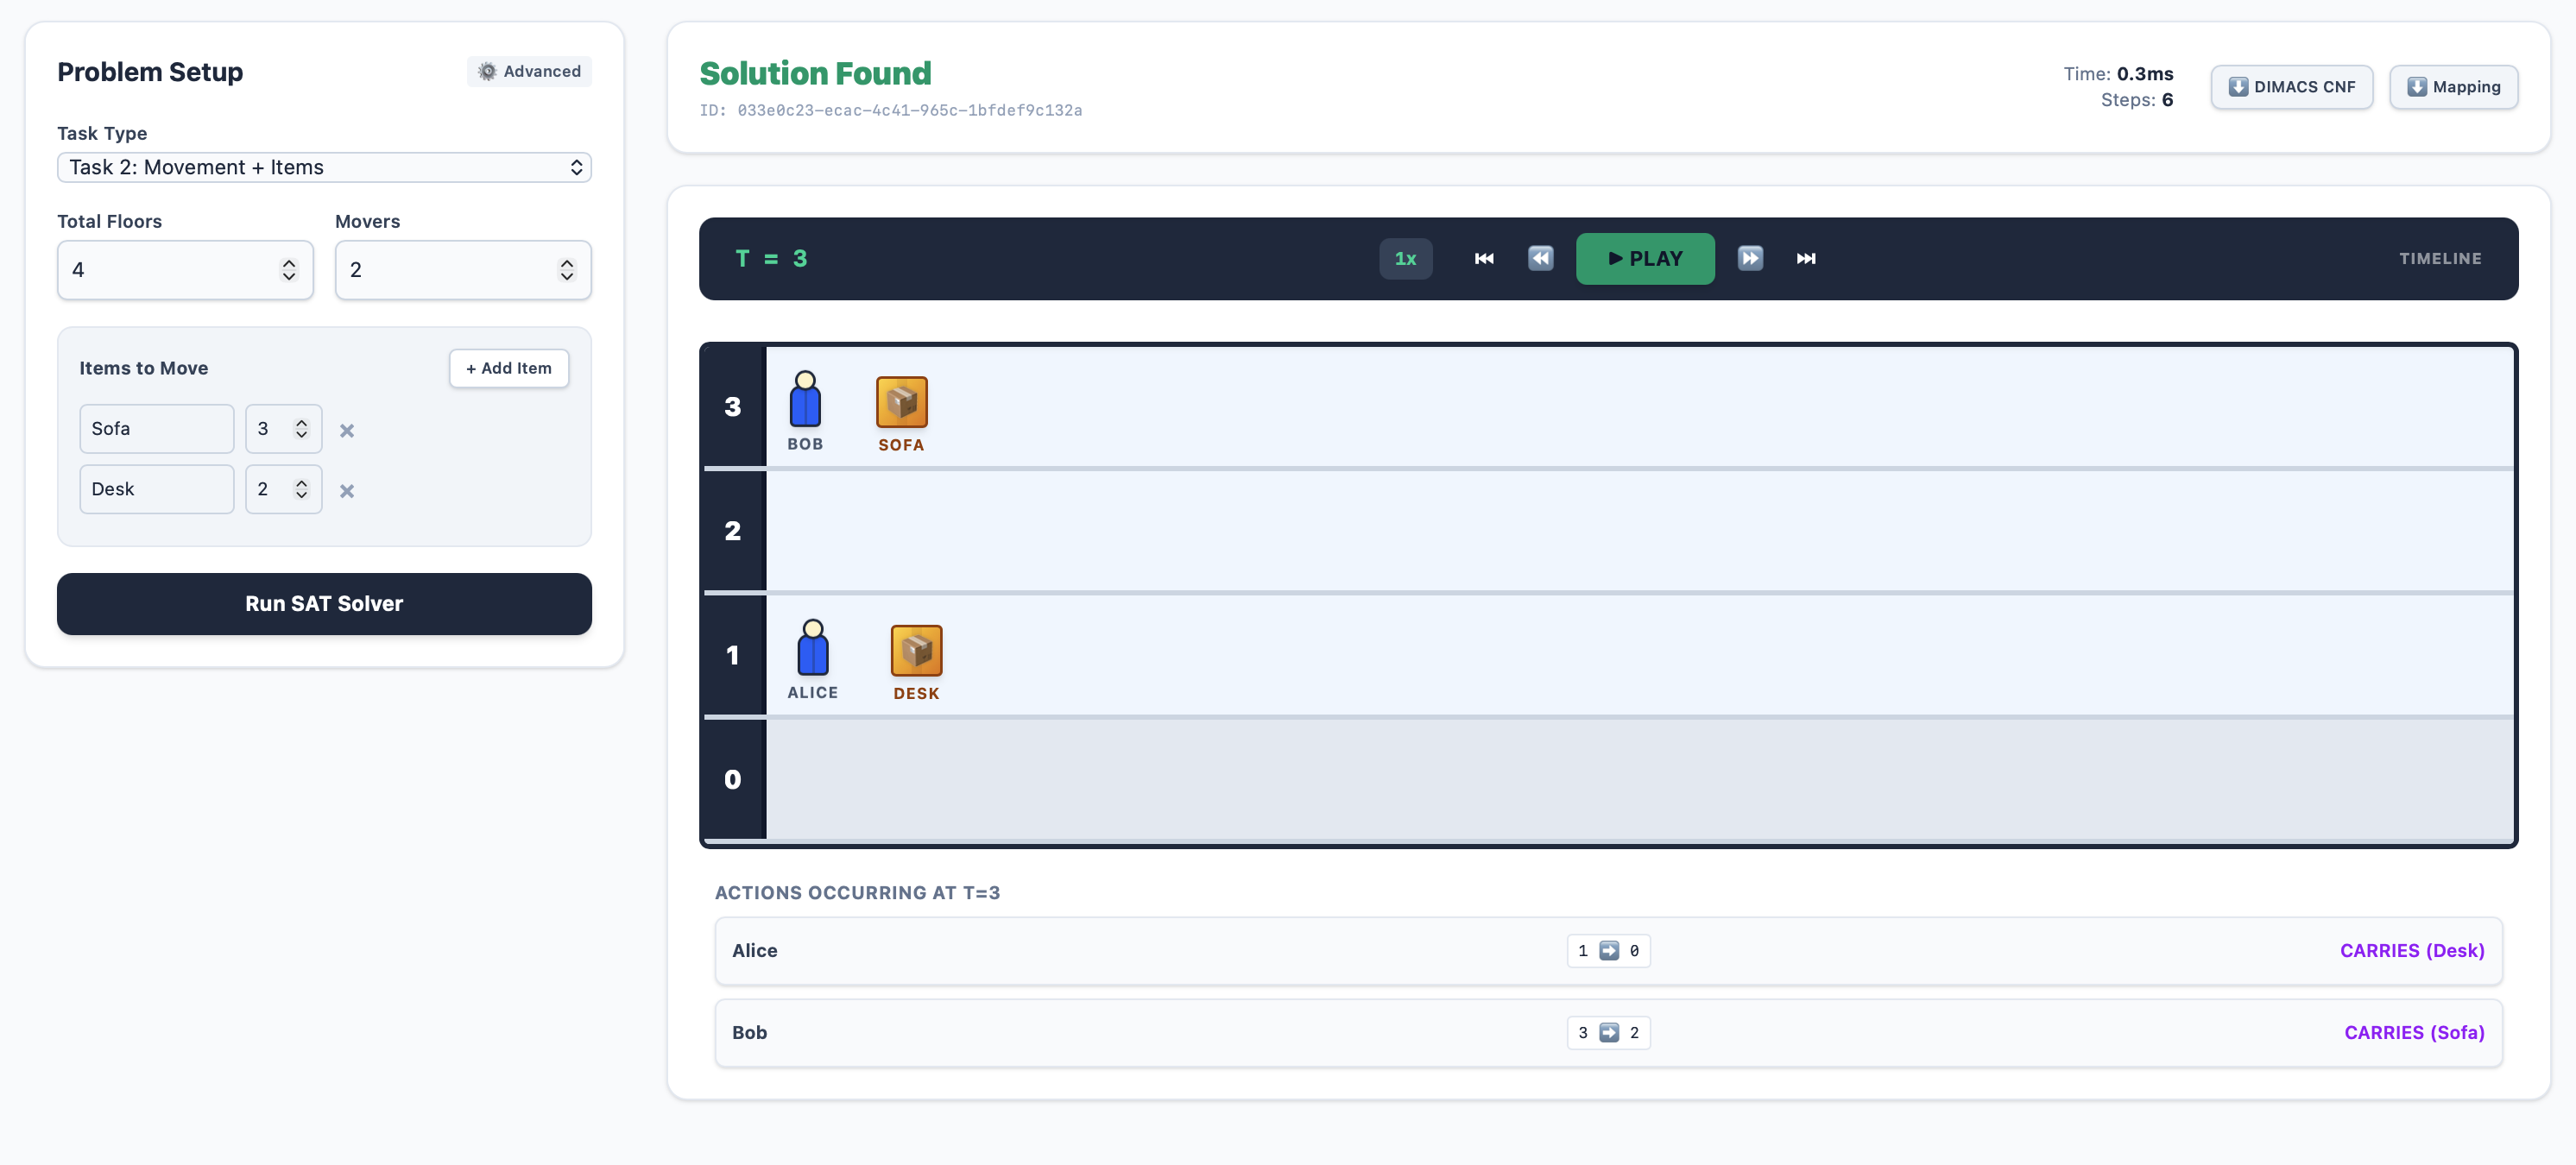
\includegraphics[width=0.95\textwidth]{img/task2-frontend-overview}
    \caption{Frontend visualization of a satisfiable Task 2 instance with two movers and two items.}
    \label{fig:frontend-sat}
\end{figure}

\subsection{Action Log}

The action log describes what happens at the selected time step.
For example, it may show that Alice descends from floor $2$ to floor $1$, or that Bob carries a table from floor $1$ to floor $0$.
    \newpage

    \section{Complexity and Scalability Analysis} \label{sec:complexity-and-scalability-analysis}
\subsection{Variable Growth} \label{subsec:variable-growth}

Let:
\begin{align*}
    n &= \text{number of floors}, \\
    m &= \text{number of movers}, \\
    k &= \text{number of items}, \\
    T &= \text{time horizon}.
\end{align*}

\noindent For Task 1, the number of variables is approximately:
\[
    m n (T+1) + 2mT.
\]
The first term represents mover positions, while the second term represents the ascend and descend action variables.

\noindent For Task 2, item positions and carrying variables are added:
\[
    m n (T+1) + k n (T+1) + 2mT + mkT.
\]

\noindent Thus, the number of variables grows linearly with the time horizon $T$, but also depends on the product $mk$ because every mover-item pair may correspond to a carrying variable at every step.

\subsection{Clause Growth} \label{subsec:clause-growth}

The largest source of clauses comes from exactly-one and at-most-one constraints.
Because the implementation uses pairwise at-most-one clauses, enforcing uniqueness over $r$ literals requires:
\[
    \binom{r}{2}
\]
binary clauses.

\noindent For example, requiring a person to be on exactly one of $n$ floors at a given time step requires:
\[
    1 + \binom{n}{2}
\]
clauses.
This is repeated for every person and every time step.

\noindent Task 2 adds similar constraints for items, as well as carrying mutex constraints between movers and items.
Therefore, the number of clauses grows polynomially in the input parameters for a fixed horizon.

\subsection{SAT Solving Complexity} \label{subsec:sat-solving-complexity}

\noindent Although the encoding size is polynomial in $n$, $m$, $k$, and $T$, SAT solving is NP-complete in the worst case.
Therefore, there is no guarantee that every large instance will be solved quickly.

\noindent In practice, modern SAT solvers such as Glucose3 exploit structure, unit propagation, clause learning, and branching heuristics.
For the tested problem sizes, the solver usually returns results within milliseconds.

\subsection{Practical Scalability} \label{subsec:practical-scalability}

The most important factor affecting performance is the chosen time horizon.
In fixed-horizon mode, an unrealistically small $T$ often produces an unsatisfiable instance quickly, while a larger $T$ may produce many more variables and clauses.
In iterative deepening mode, the backend solves a sequence of formulas, which is useful for optimality but can become expensive when the optimal plan requires many steps.
    \newpage

    \section{Experimental Evaluation} \label{sec:experimental-evaluation}
This section describes the main test cases used to evaluate the solver.

\subsection{Case 1: Task 1 Movement with Different Goal Floors} \label{subsec:case-1:-task-1-movement-with-different-goal-floors}

For the movement-only task, three movers start on floor $0$:
\[
    \texttt{atFloor(Alice,0,0)}, \quad
    \texttt{atFloor(Bob,0,0)}, \quad
    \texttt{atFloor(Eve,0,0)}.
\]

\noindent In the tested configuration, the building has seven floors and the target floors are:
\[
    \texttt{Alice}@6, \qquad \texttt{Bob}@4, \qquad \texttt{Eve}@2.
\]

\noindent The solver finds an optimal plan in six steps.
This is expected because Alice must ascend from floor $0$ to floor $6$, which requires six upward movements.
Bob and Eve reach their target floors earlier and then remain idle while Alice completes the longest path.

\begin{figure}[H]
    \centering
    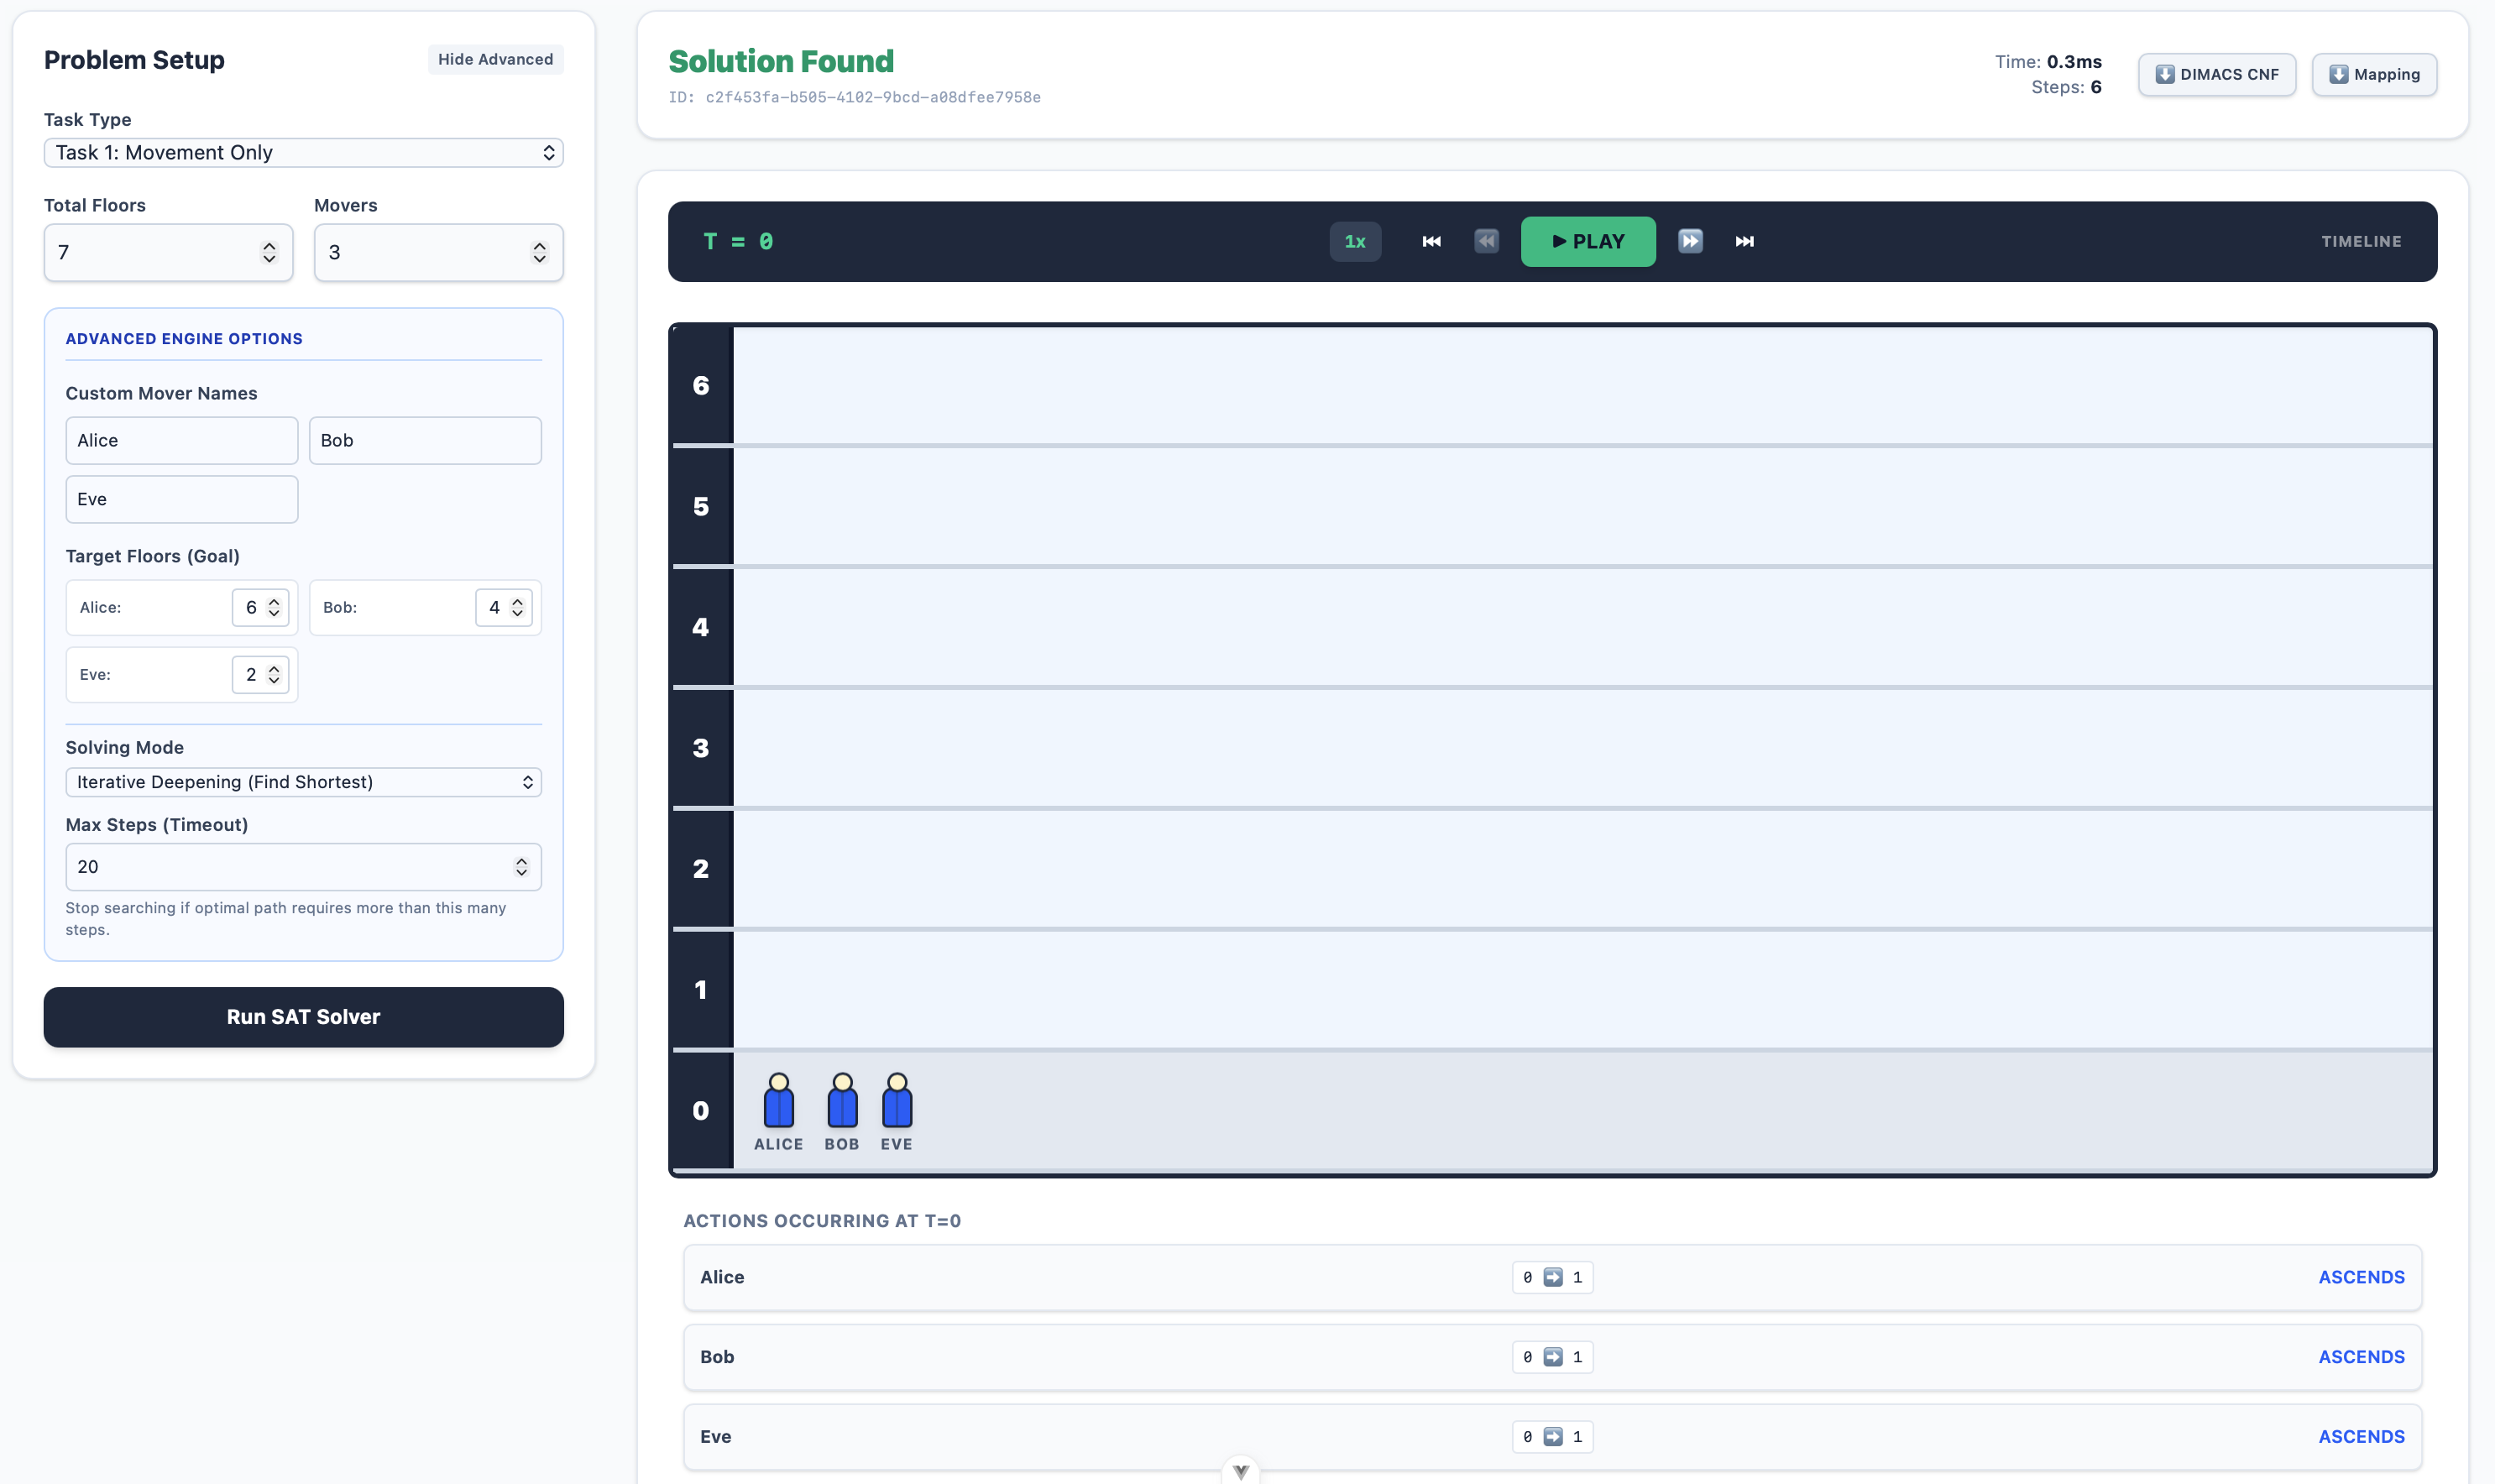
\includegraphics[width=0.95\textwidth]{img/task1-initial-state}
    \caption{Initial state of a Task 1 instance: all movers start on the ground floor.}
    \label{fig:task1-initial}
\end{figure}

\begin{figure}[H]
    \centering
    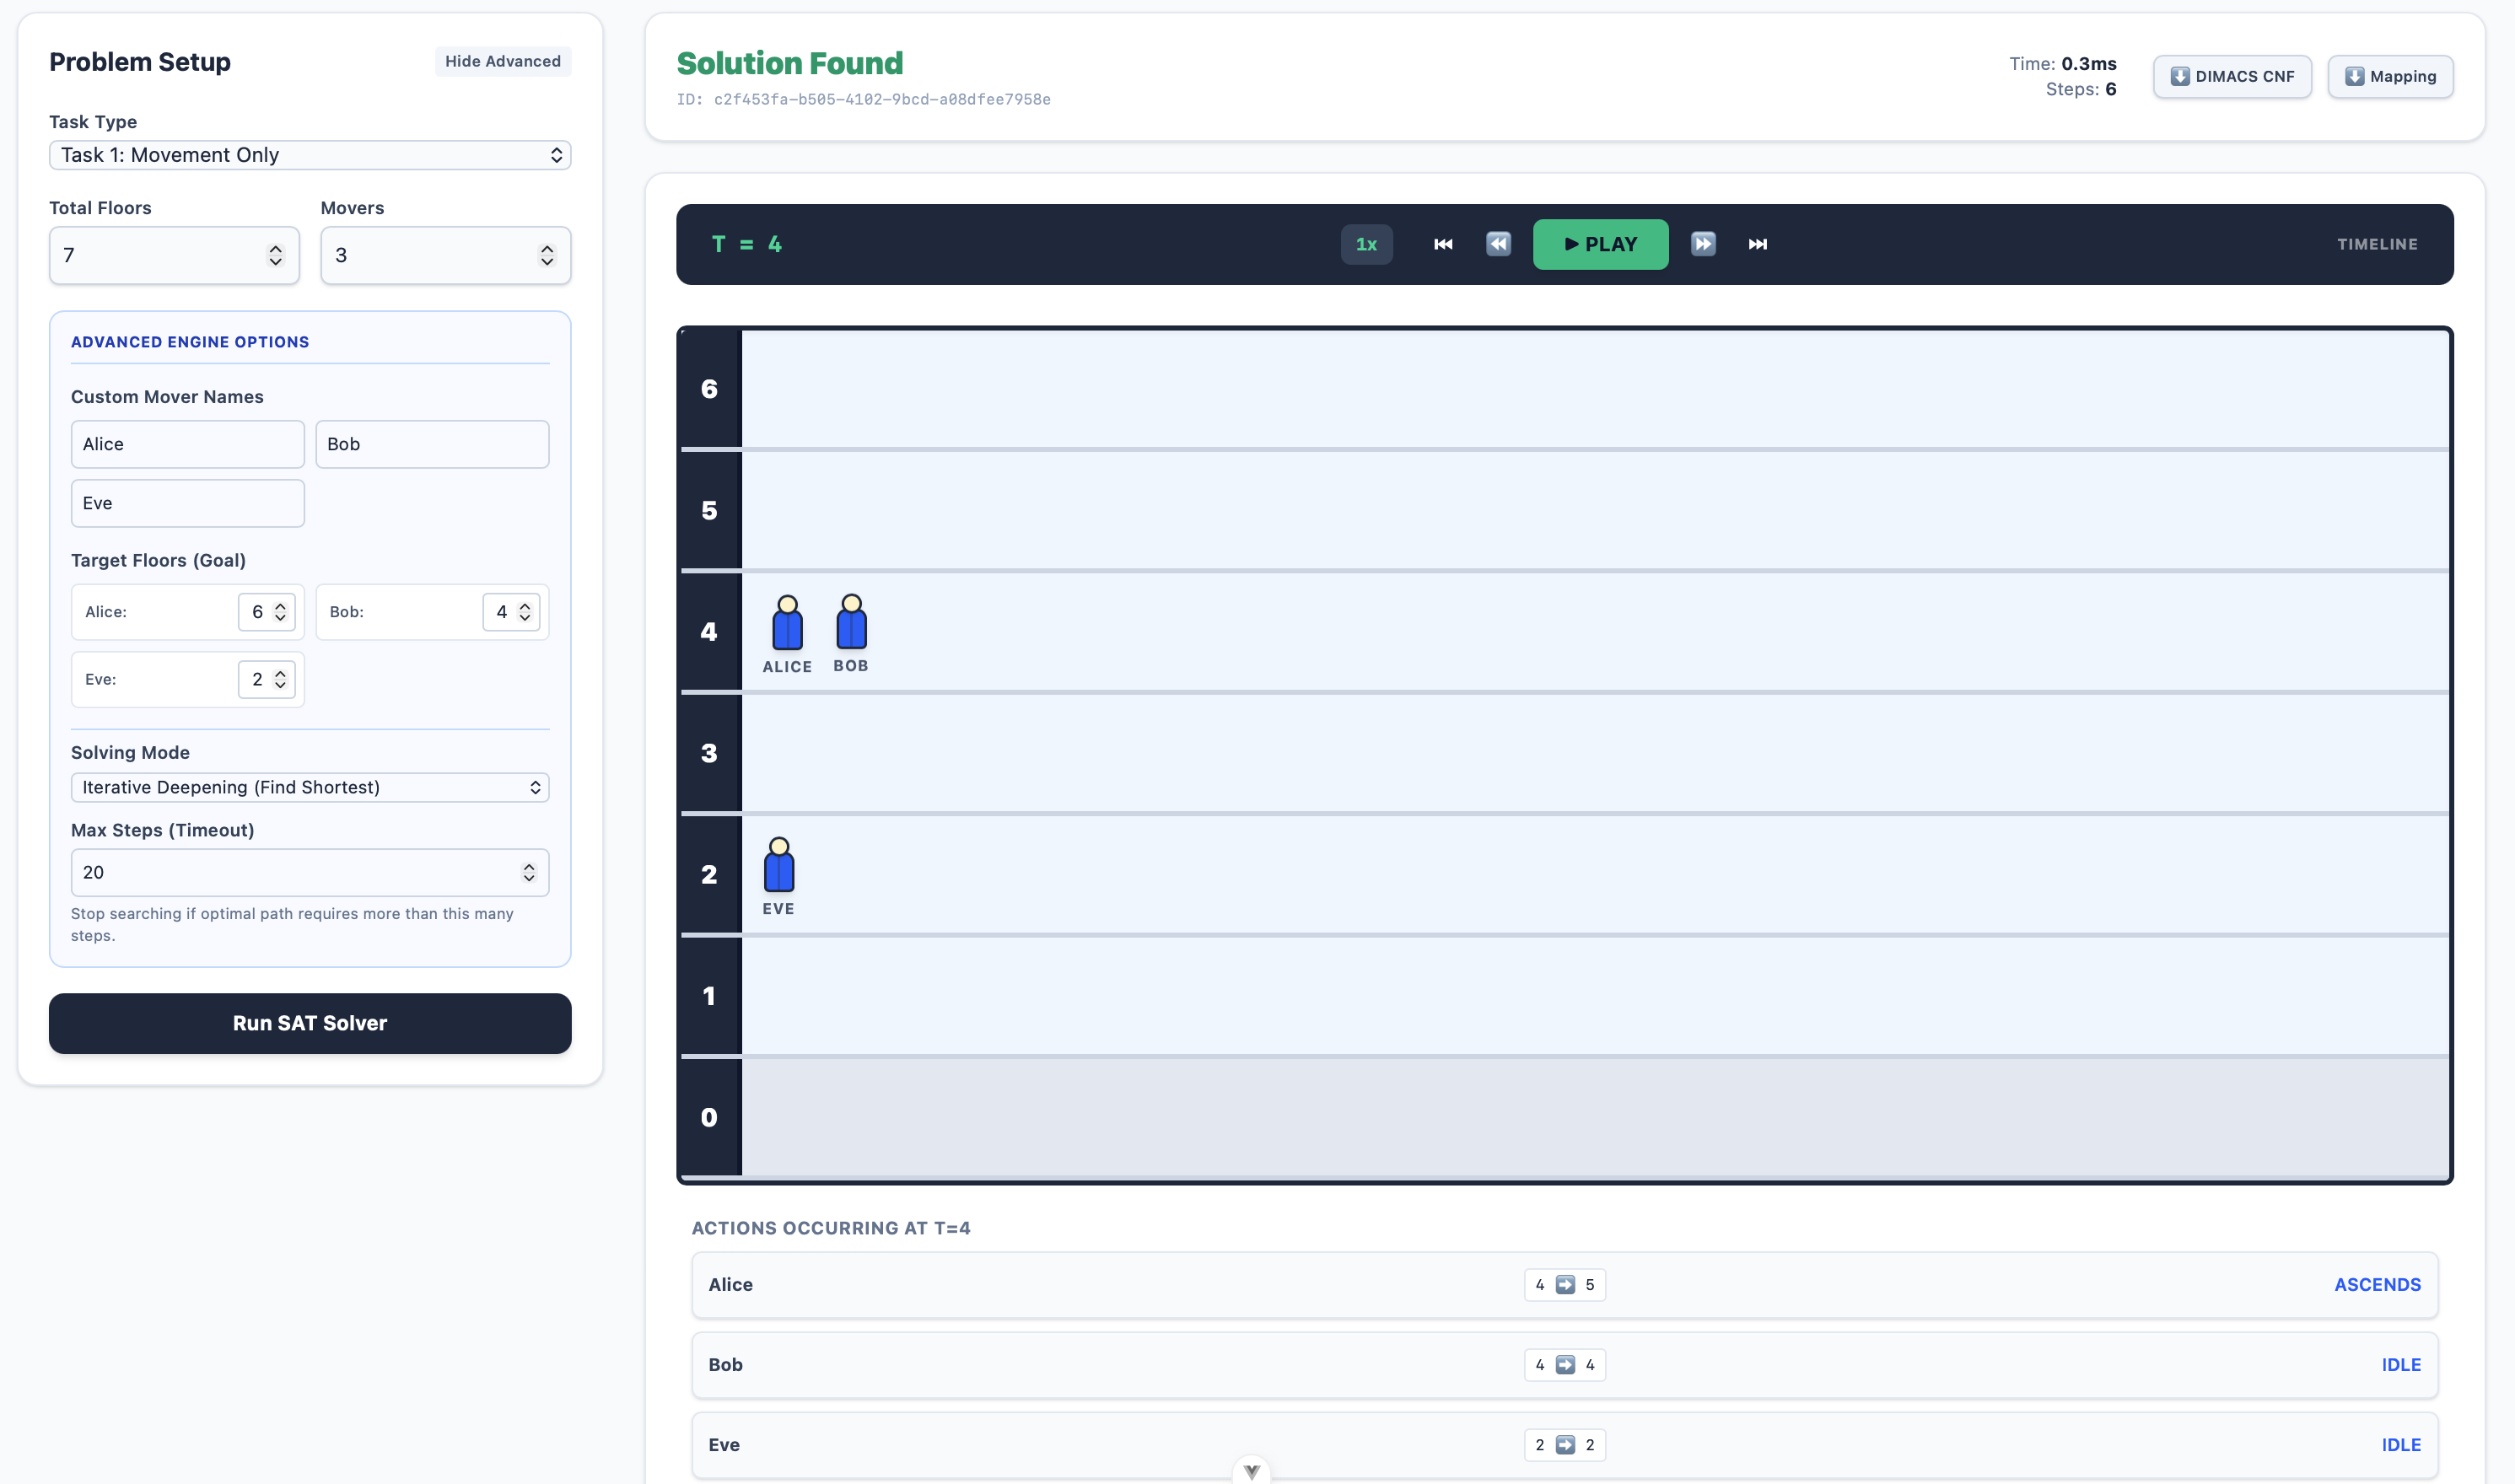
\includegraphics[width=0.95\textwidth]{img/task1-intermediate-state}
    \caption{Intermediate state of the Task 1 solution, where some movers have already reached their target floors.}
    \label{fig:task1-middle}
\end{figure}

\begin{figure}[H]
    \centering
    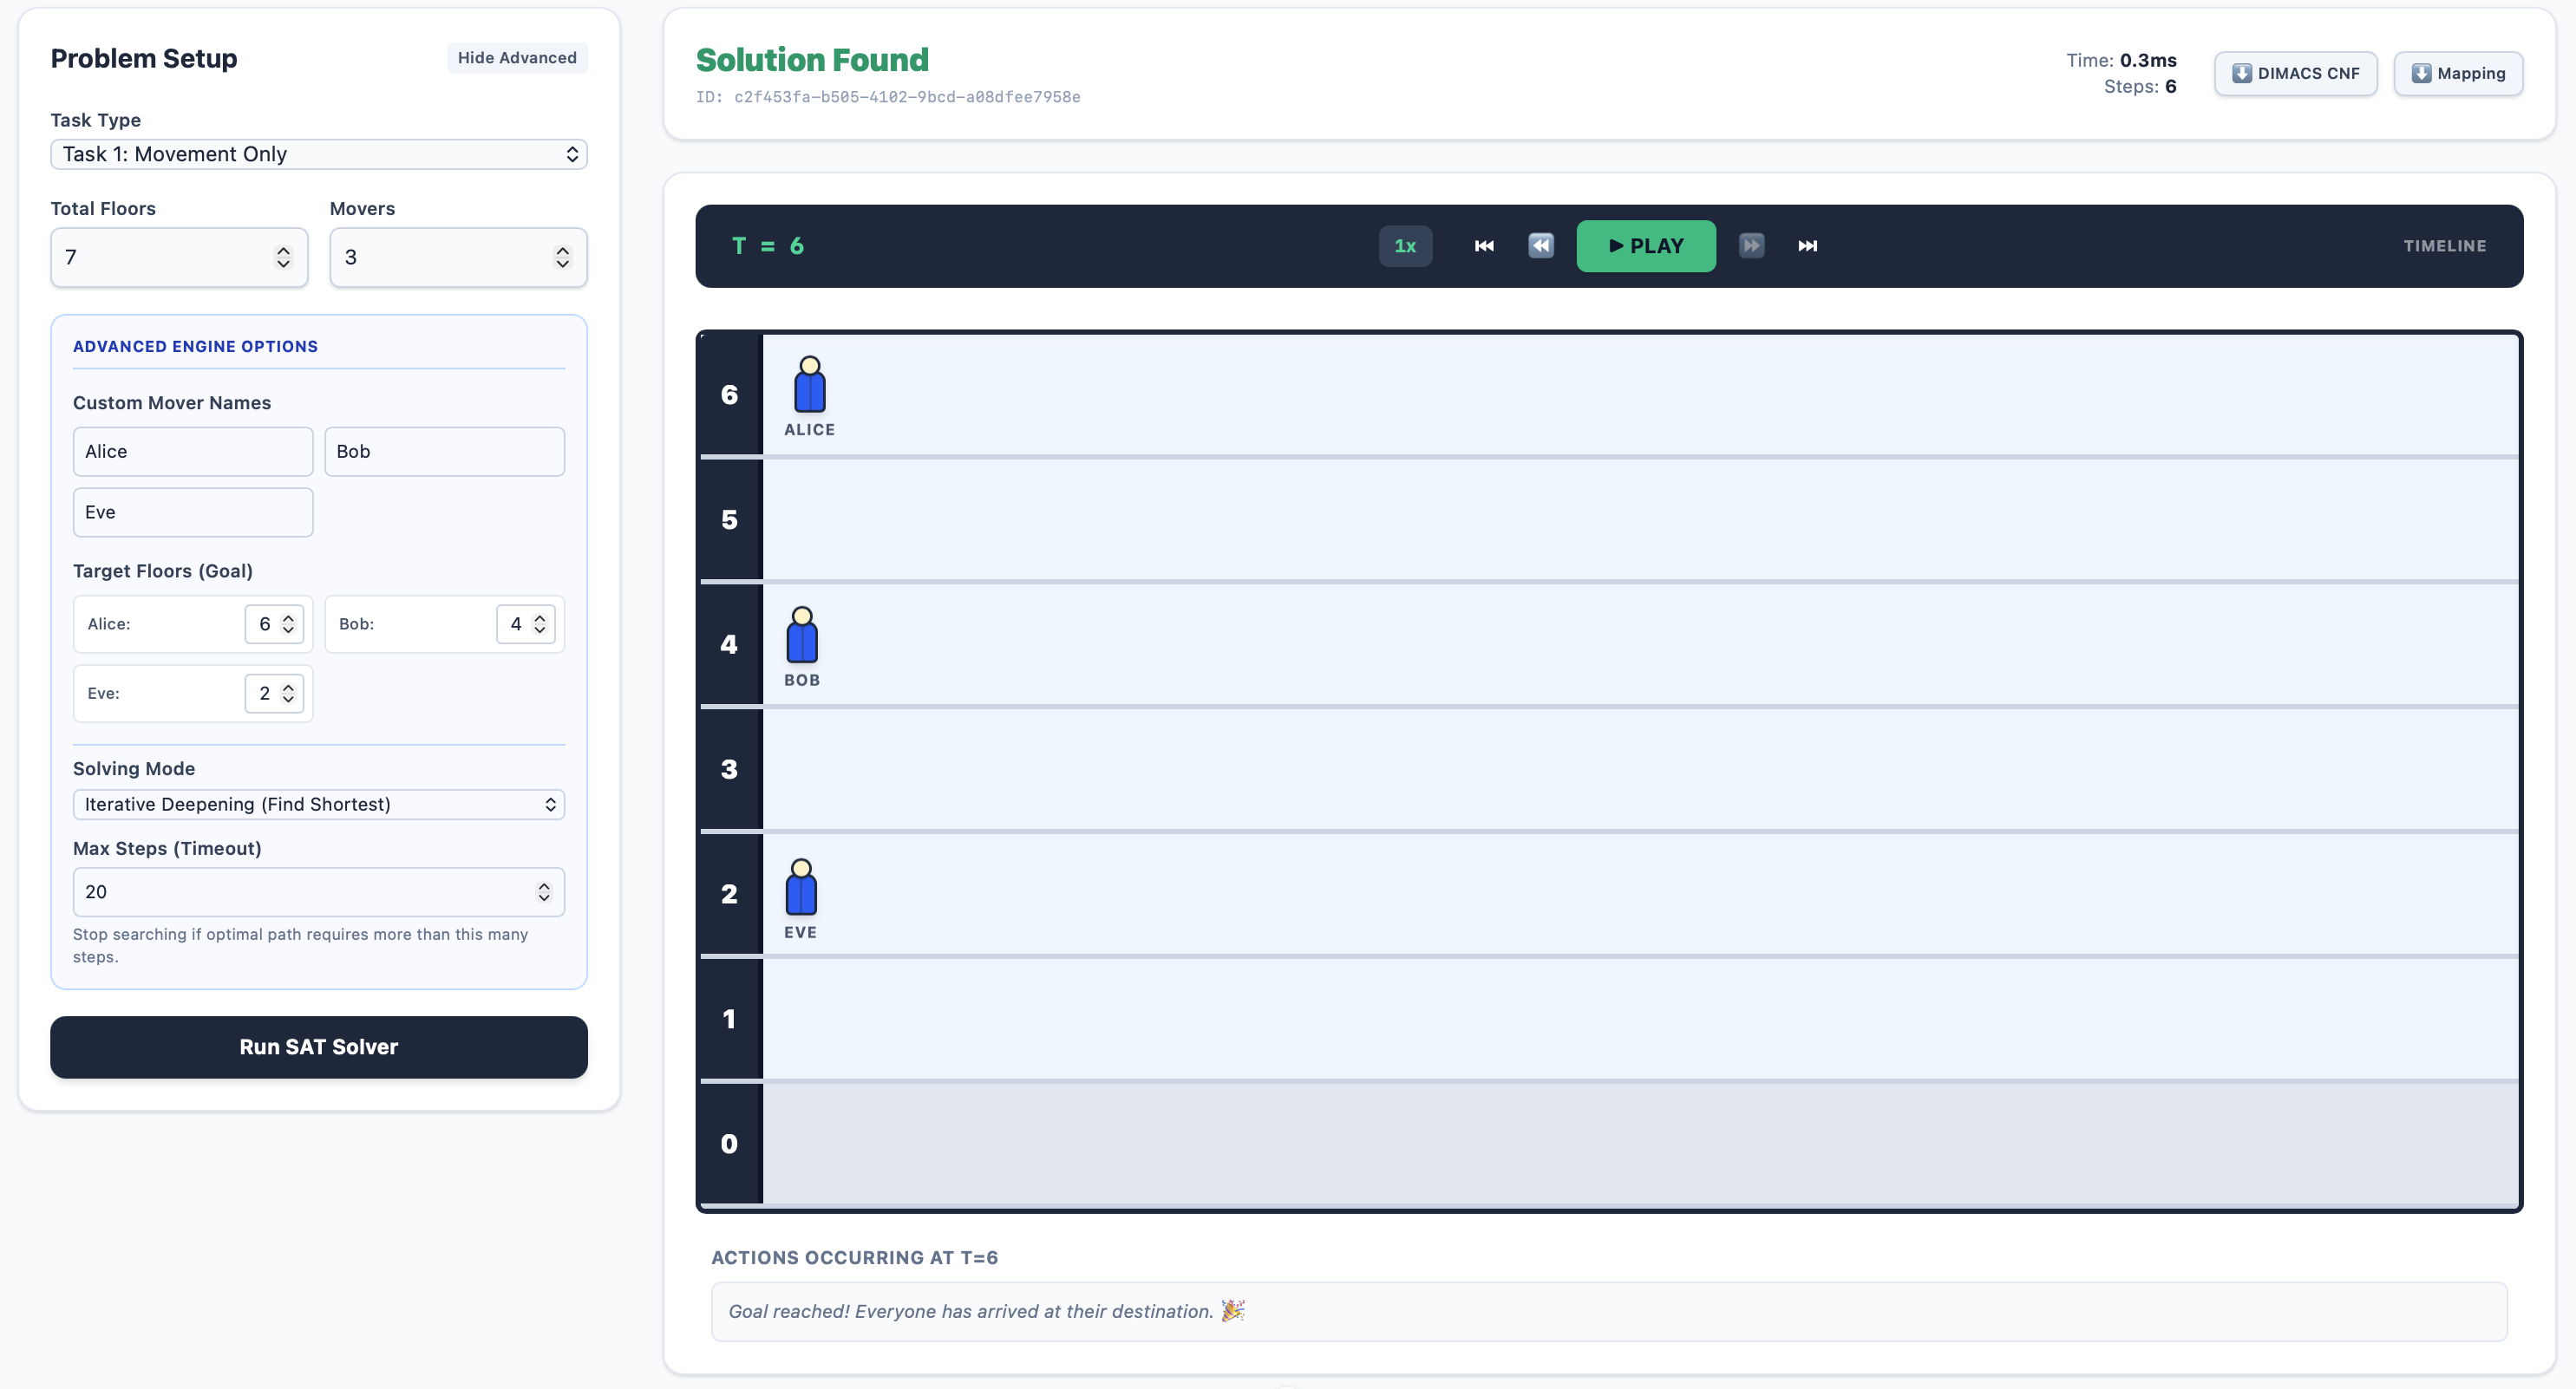
\includegraphics[width=0.95\textwidth]{img/task1-final-state}
    \caption{Final state of the Task 1 solution: Alice, Bob, and Eve are on their required target floors.}
    \label{fig:task1-final}
\end{figure}

\subsection{Case 2: Task 1 Unsatisfiable Within a Limited Horizon} \label{subsec:case-2:-task-1-unsatisfiable-within-a-limited-horizon}

The same Task 1 goal cannot be reached if the maximum allowed time horizon is too small.
For example, Alice must reach floor $6$ from floor $0$, so any solution requires at least six time steps.
If the search is stopped at $T_{\max}=4$, the solver correctly reports the instance as unsatisfiable within the given bound.

\begin{figure}[H]
    \centering
    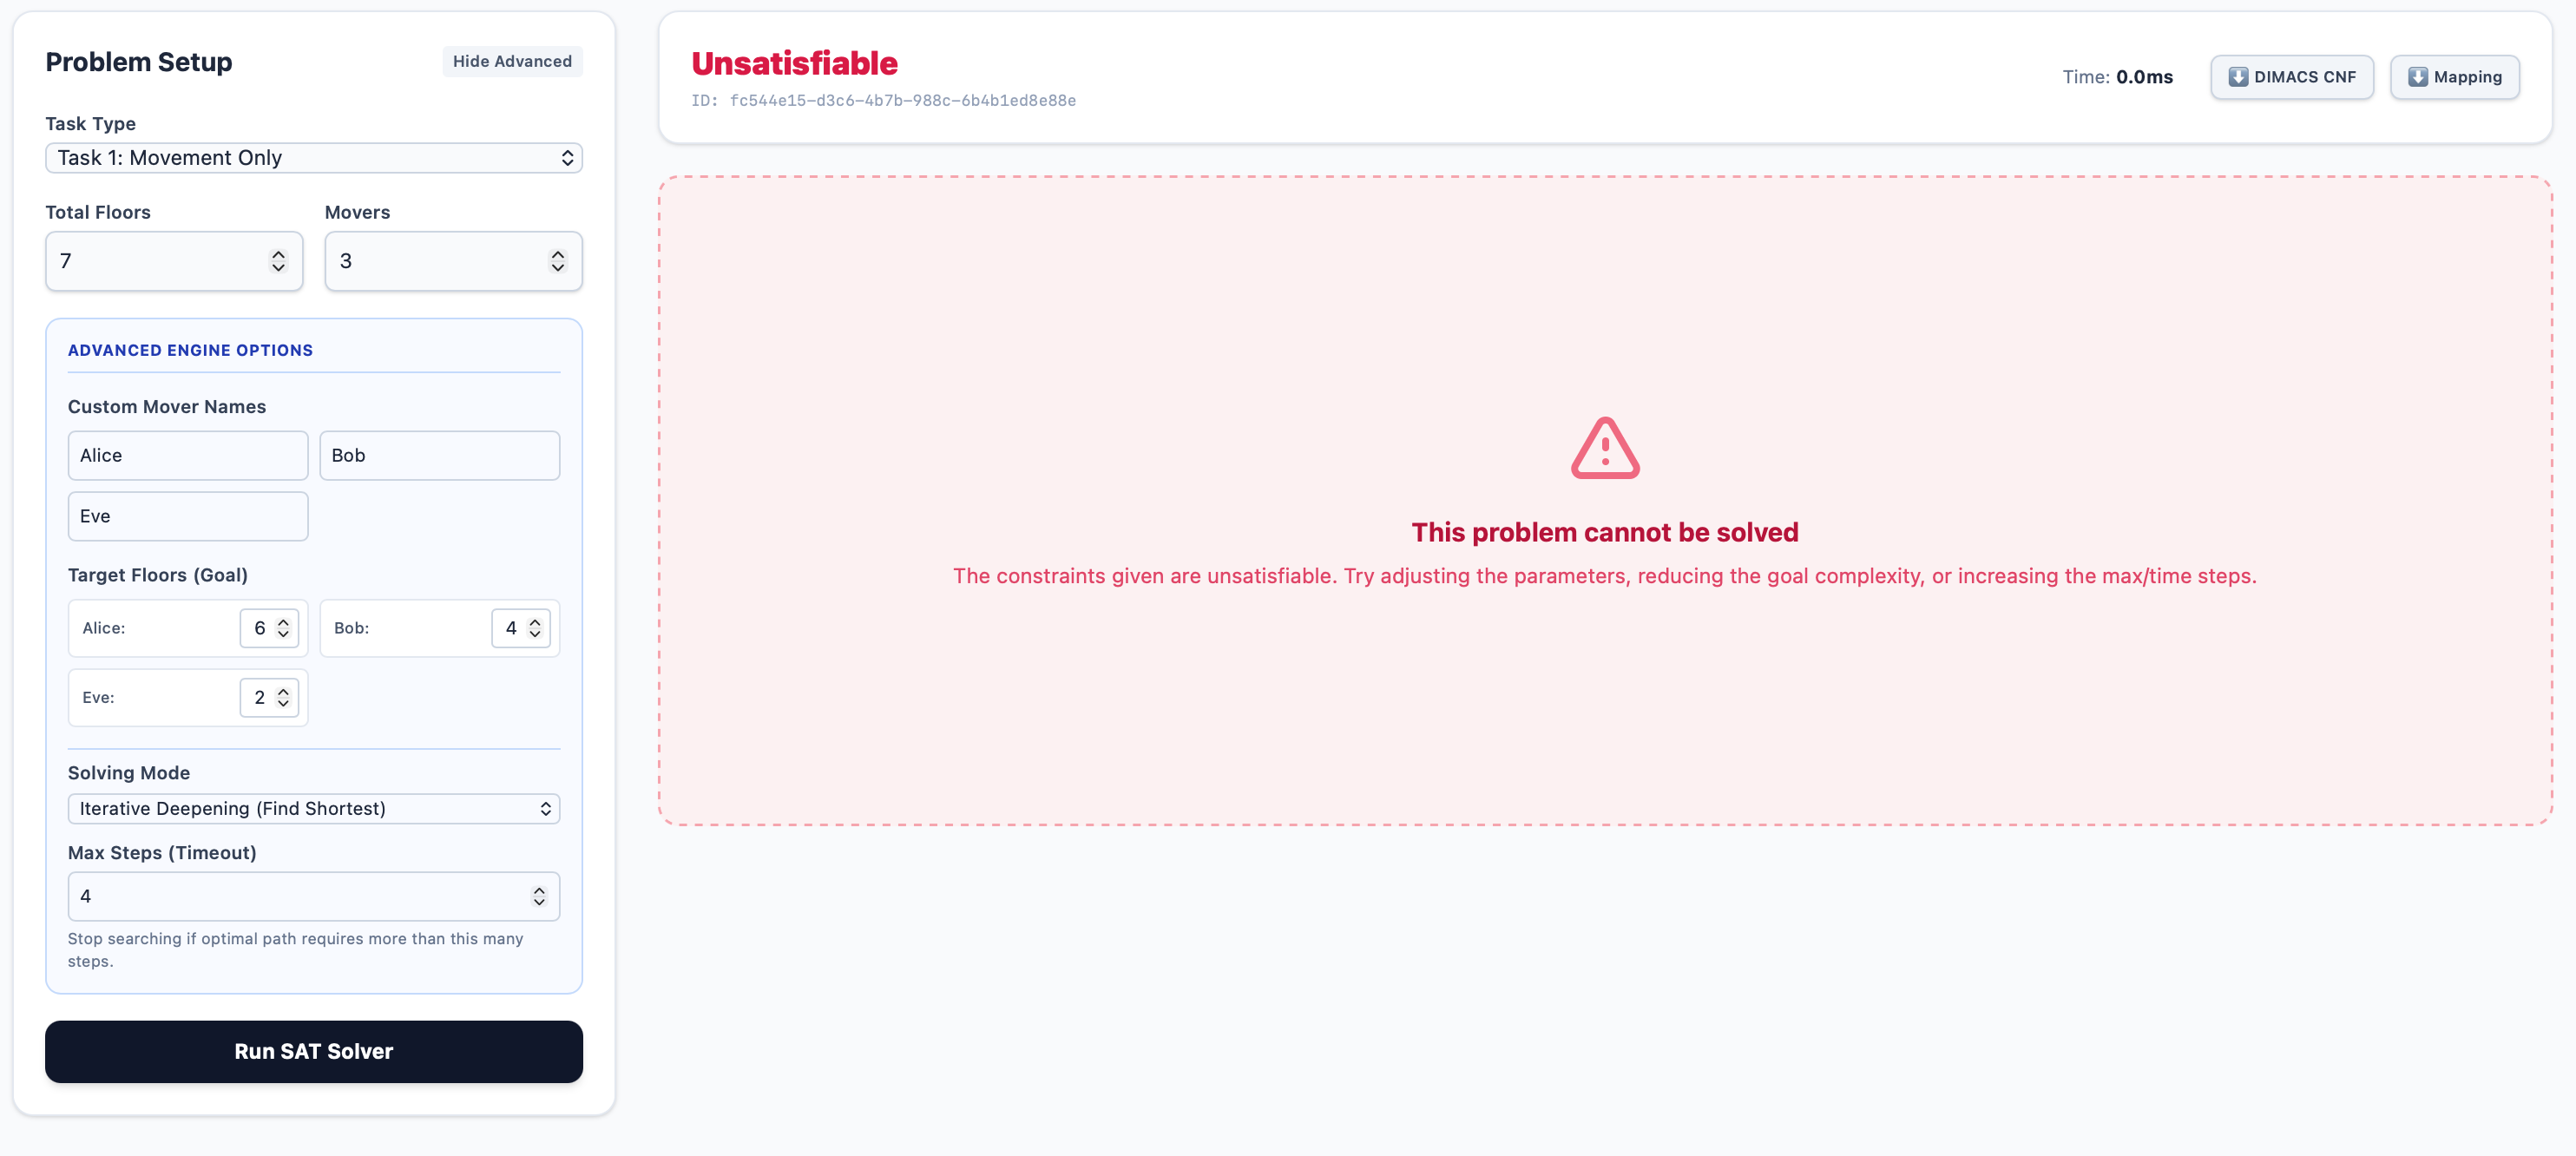
\includegraphics[width=0.95\textwidth]{img/task1-unsat-result}
    \caption{Task 1 unsatisfiable result when the maximum search horizon is too small to reach the target floors.}
    \label{fig:task1-unsat}
\end{figure}

\subsection{Case 3: Trivial Task 1 Goal} \label{subsec:case-3:-trivial-task-1-goal}

If the target floor is already floor $0$, then the initial state satisfies the goal.
The solver correctly returns a satisfiable result at $T=0$.

\subsection{Case 4: Task 2 with Three Items} \label{subsec:case-4:-task-2-with-three-items}

For the carrying task, a tested configuration uses three movers and three items:
\[
    \texttt{flowerpot}@2, \qquad
    \texttt{chair}@1, \qquad
    \texttt{table}@2.
\]

\noindent The solver finds a valid plan in four steps.
The final state places all movers and all items on floor $0$.

\subsection{Case 5: Task 2 Unsatisfiable Fixed-Horizon Instance} \label{subsec:case-5:-task-2-unsatisfiable-fixed-horizon-instance}

In this frontend test, the building has seven floors, two movers, and three items:
\[
    \texttt{Sofa}@3,\qquad
    \texttt{Desk}@4,\qquad
    \texttt{Chair}@6.
\]

\noindent The solver is executed in fixed-horizon mode with an exact time horizon of $T=10$.
The instance is reported as unsatisfiable, showing that the system correctly detects when no valid plan exists within the selected number of time steps.
This also confirms that the frontend properly displays bounded UNSAT results returned by the backend.


\begin{figure}[H]
    \centering
    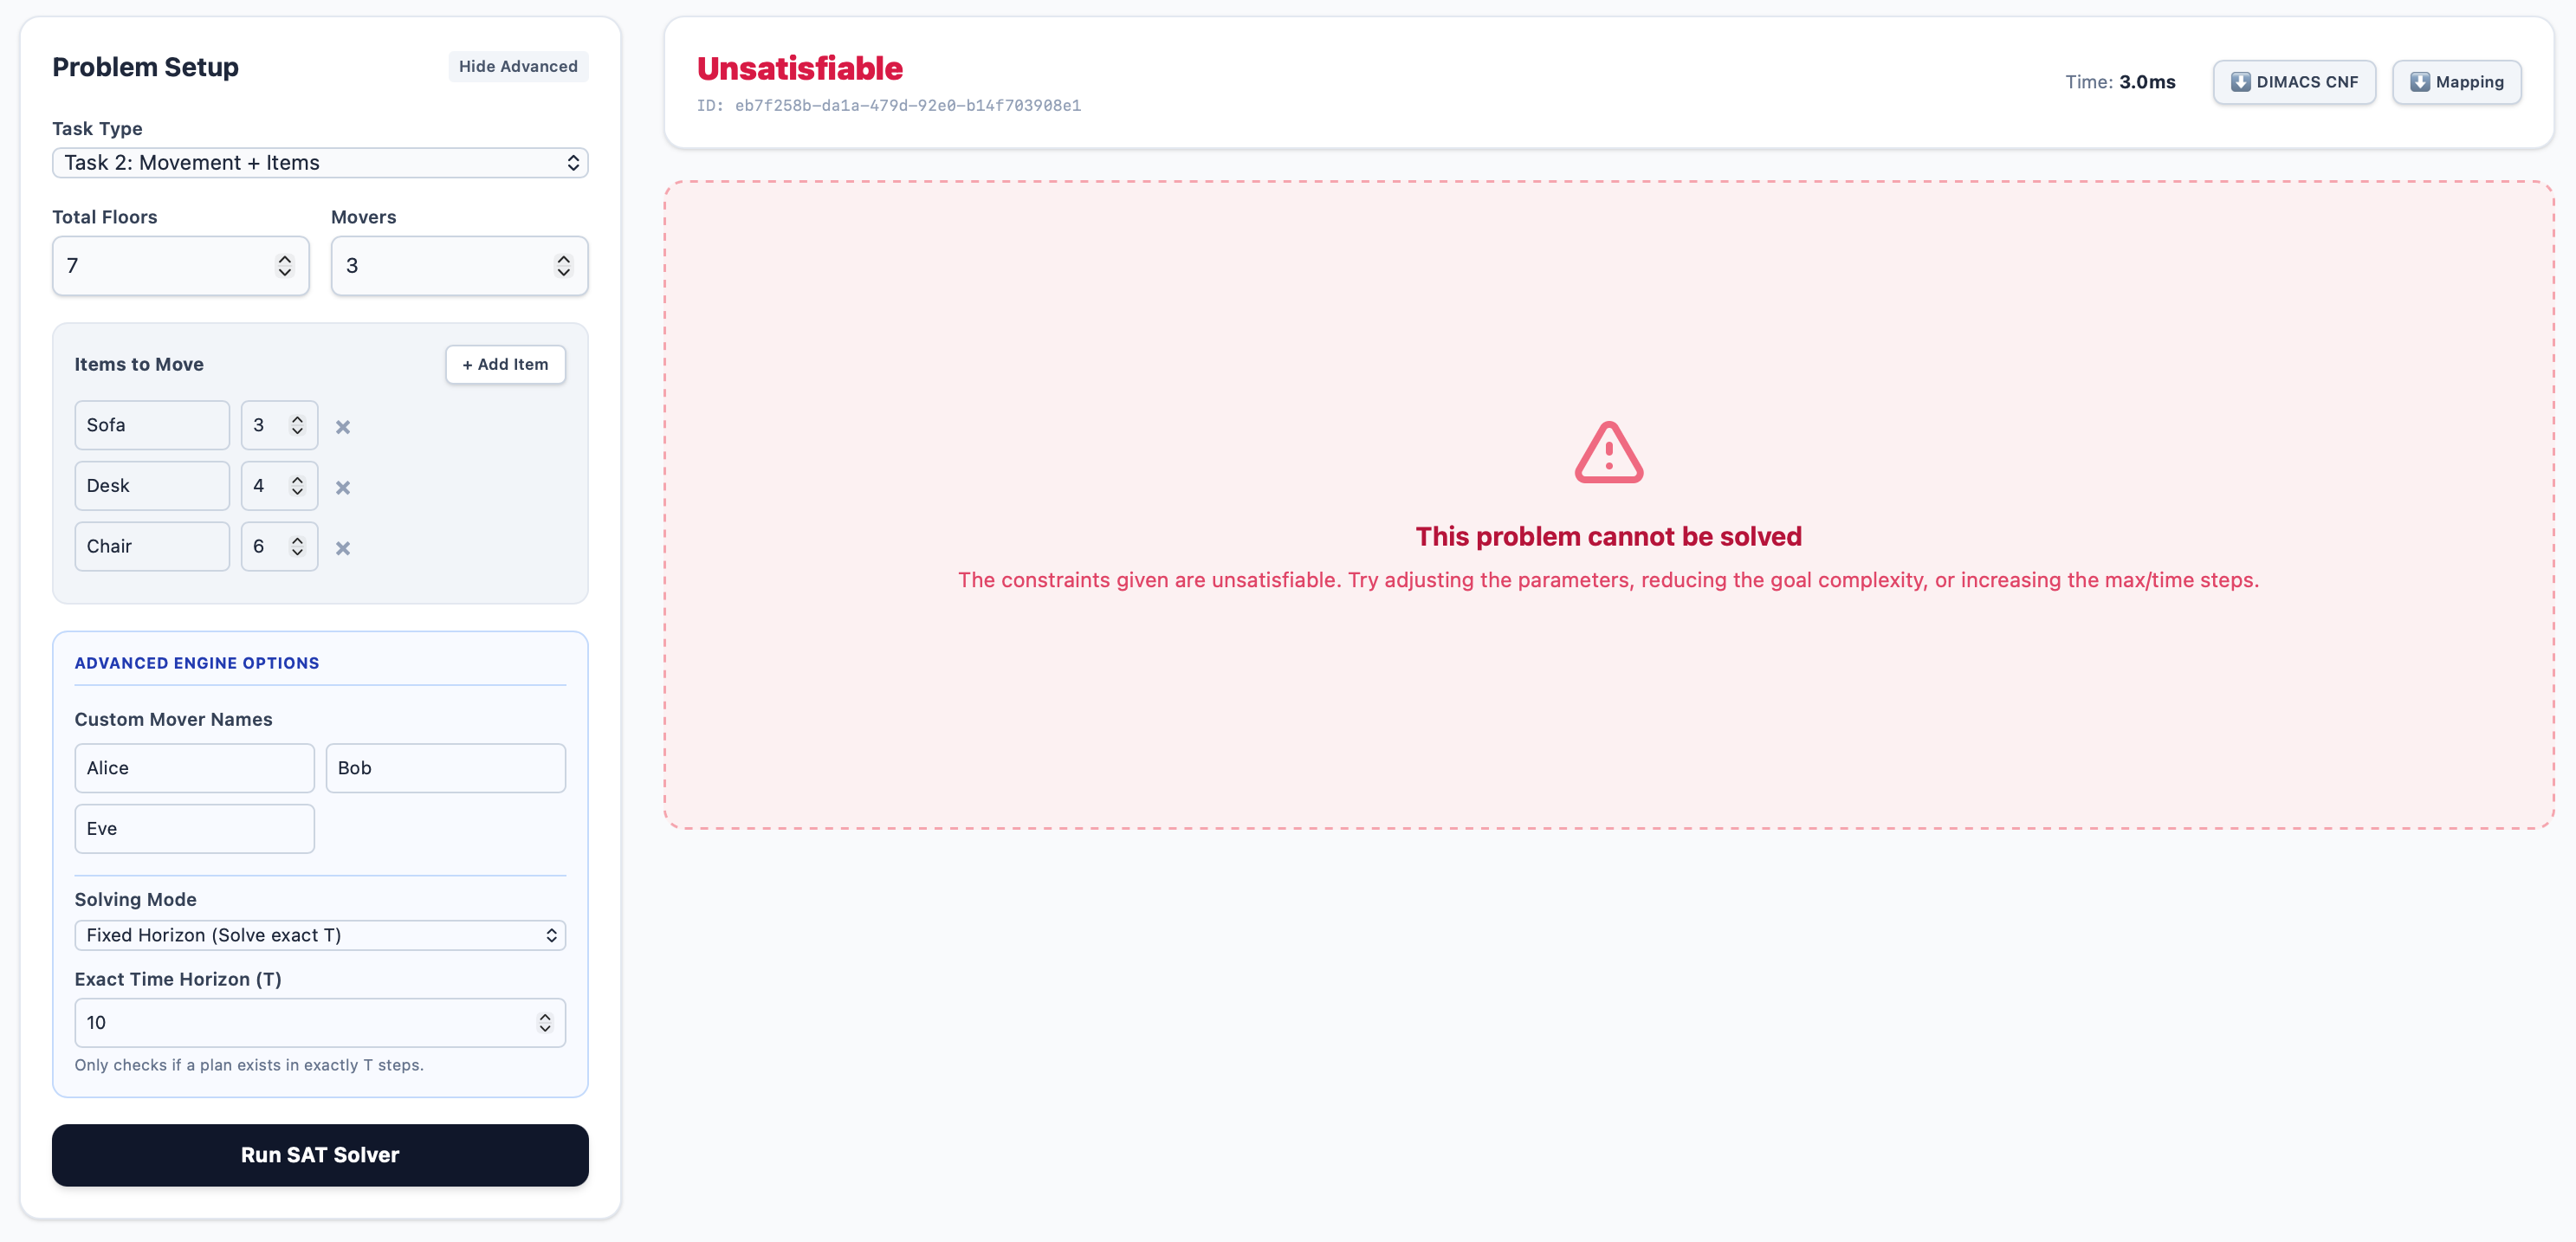
\includegraphics[width=0.95\textwidth]{img/task2-fixed-unsat}
    \caption{Frontend output for an unsatisfiable fixed-horizon Task 2 instance.}
    \label{fig:frontend-unsat}
\end{figure}

\subsection{Case 6: Full Example with Five Items} \label{subsec:case-6:-full-example-with-five-items}

The full example configuration contains:
\[
    \texttt{flowerpot}@2,\quad
    \texttt{chair}@1,\quad
    \texttt{table}@2,\quad
    \texttt{piano}@1,\quad
    \texttt{sofa}@2.
\]

\noindent The solver finds an optimal solution in six steps for this full configuration.
This confirms that the Task 2 encoding scales beyond the minimal three-item example.

\subsection{Case 7: Larger Custom Frontend Instance} \label{subsec:case-7:-larger-custom-frontend-instance}

A larger frontend example uses seven floors, three movers, and four items:
\[
    \texttt{Sofa}@3,\quad
    \texttt{Desk}@4,\quad
    \texttt{Chair}@6,\quad
    \texttt{Table}@1.
\]

\noindent The frontend visualization shows the movers and items progressing through the building until every object reaches floor $0$.
The solution is displayed with a timeline, action log, and final confirmation message.

\begin{figure}[H]
    \centering
    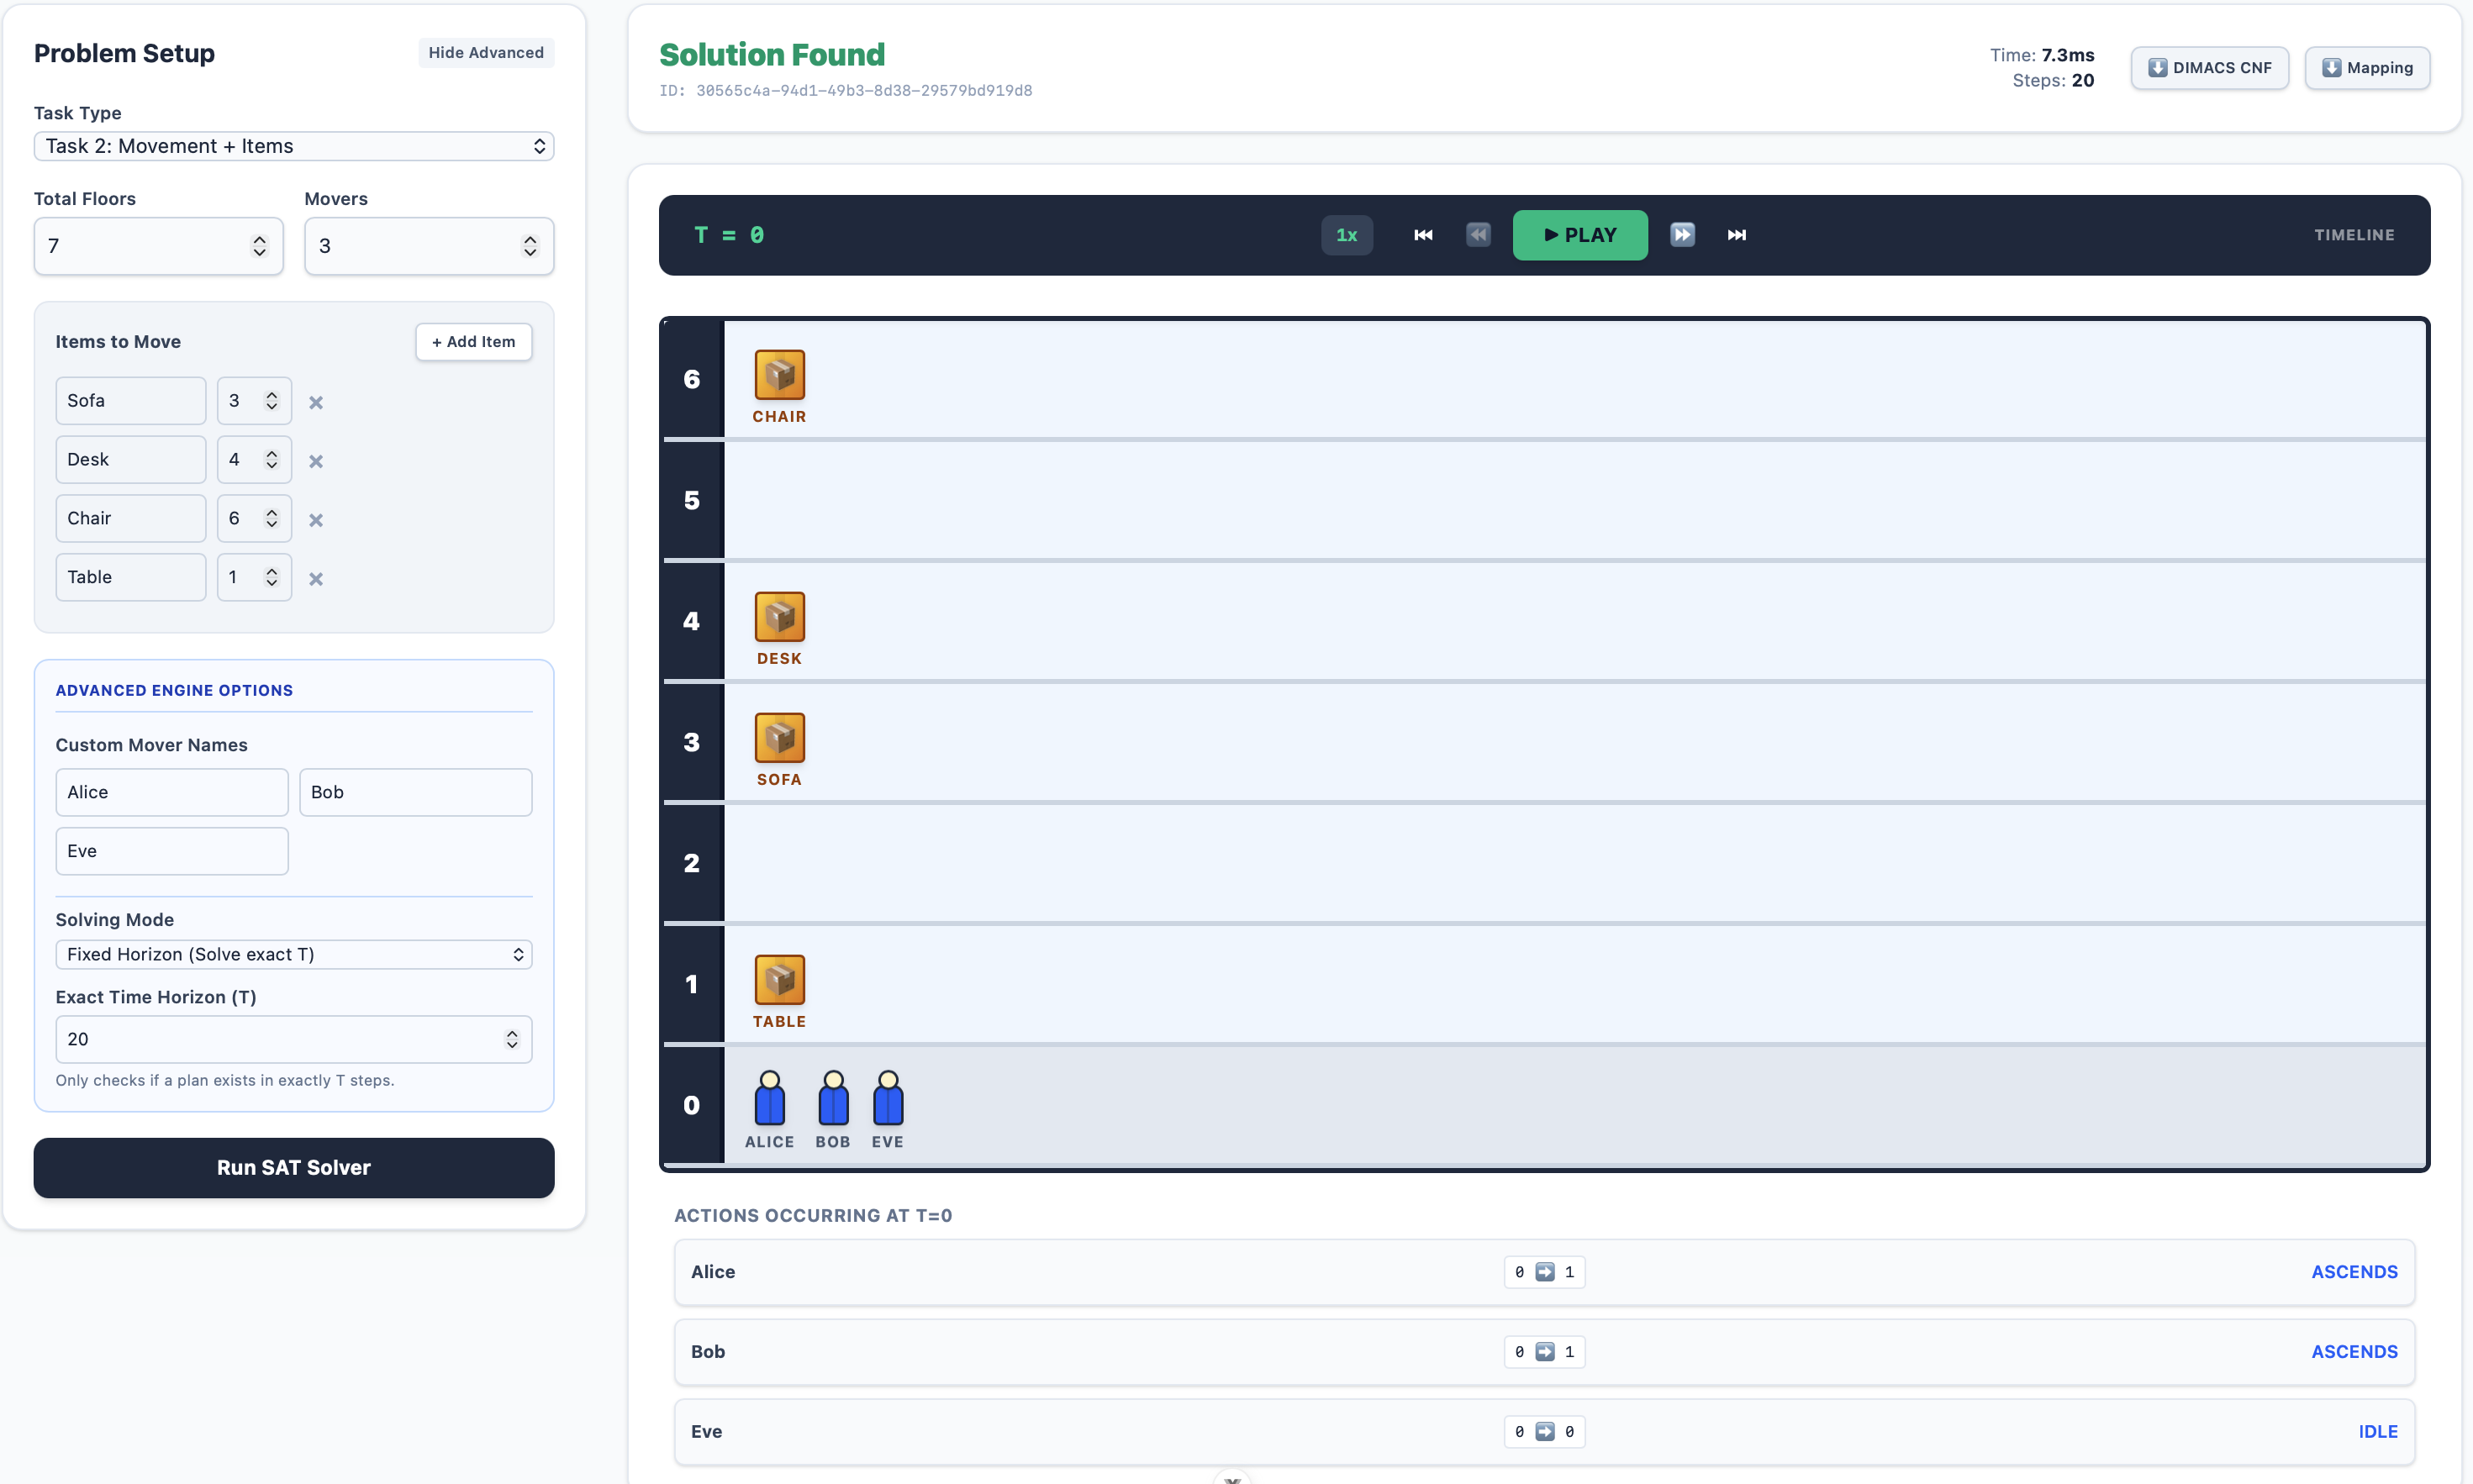
\includegraphics[width=0.95\textwidth]{img/task2-large-initial}
    \caption{Initial state of a larger Task 2 instance with seven floors, three movers, and four items.}
    \label{fig:large-instance-initial}
\end{figure}

\begin{figure}[H]
    \centering
    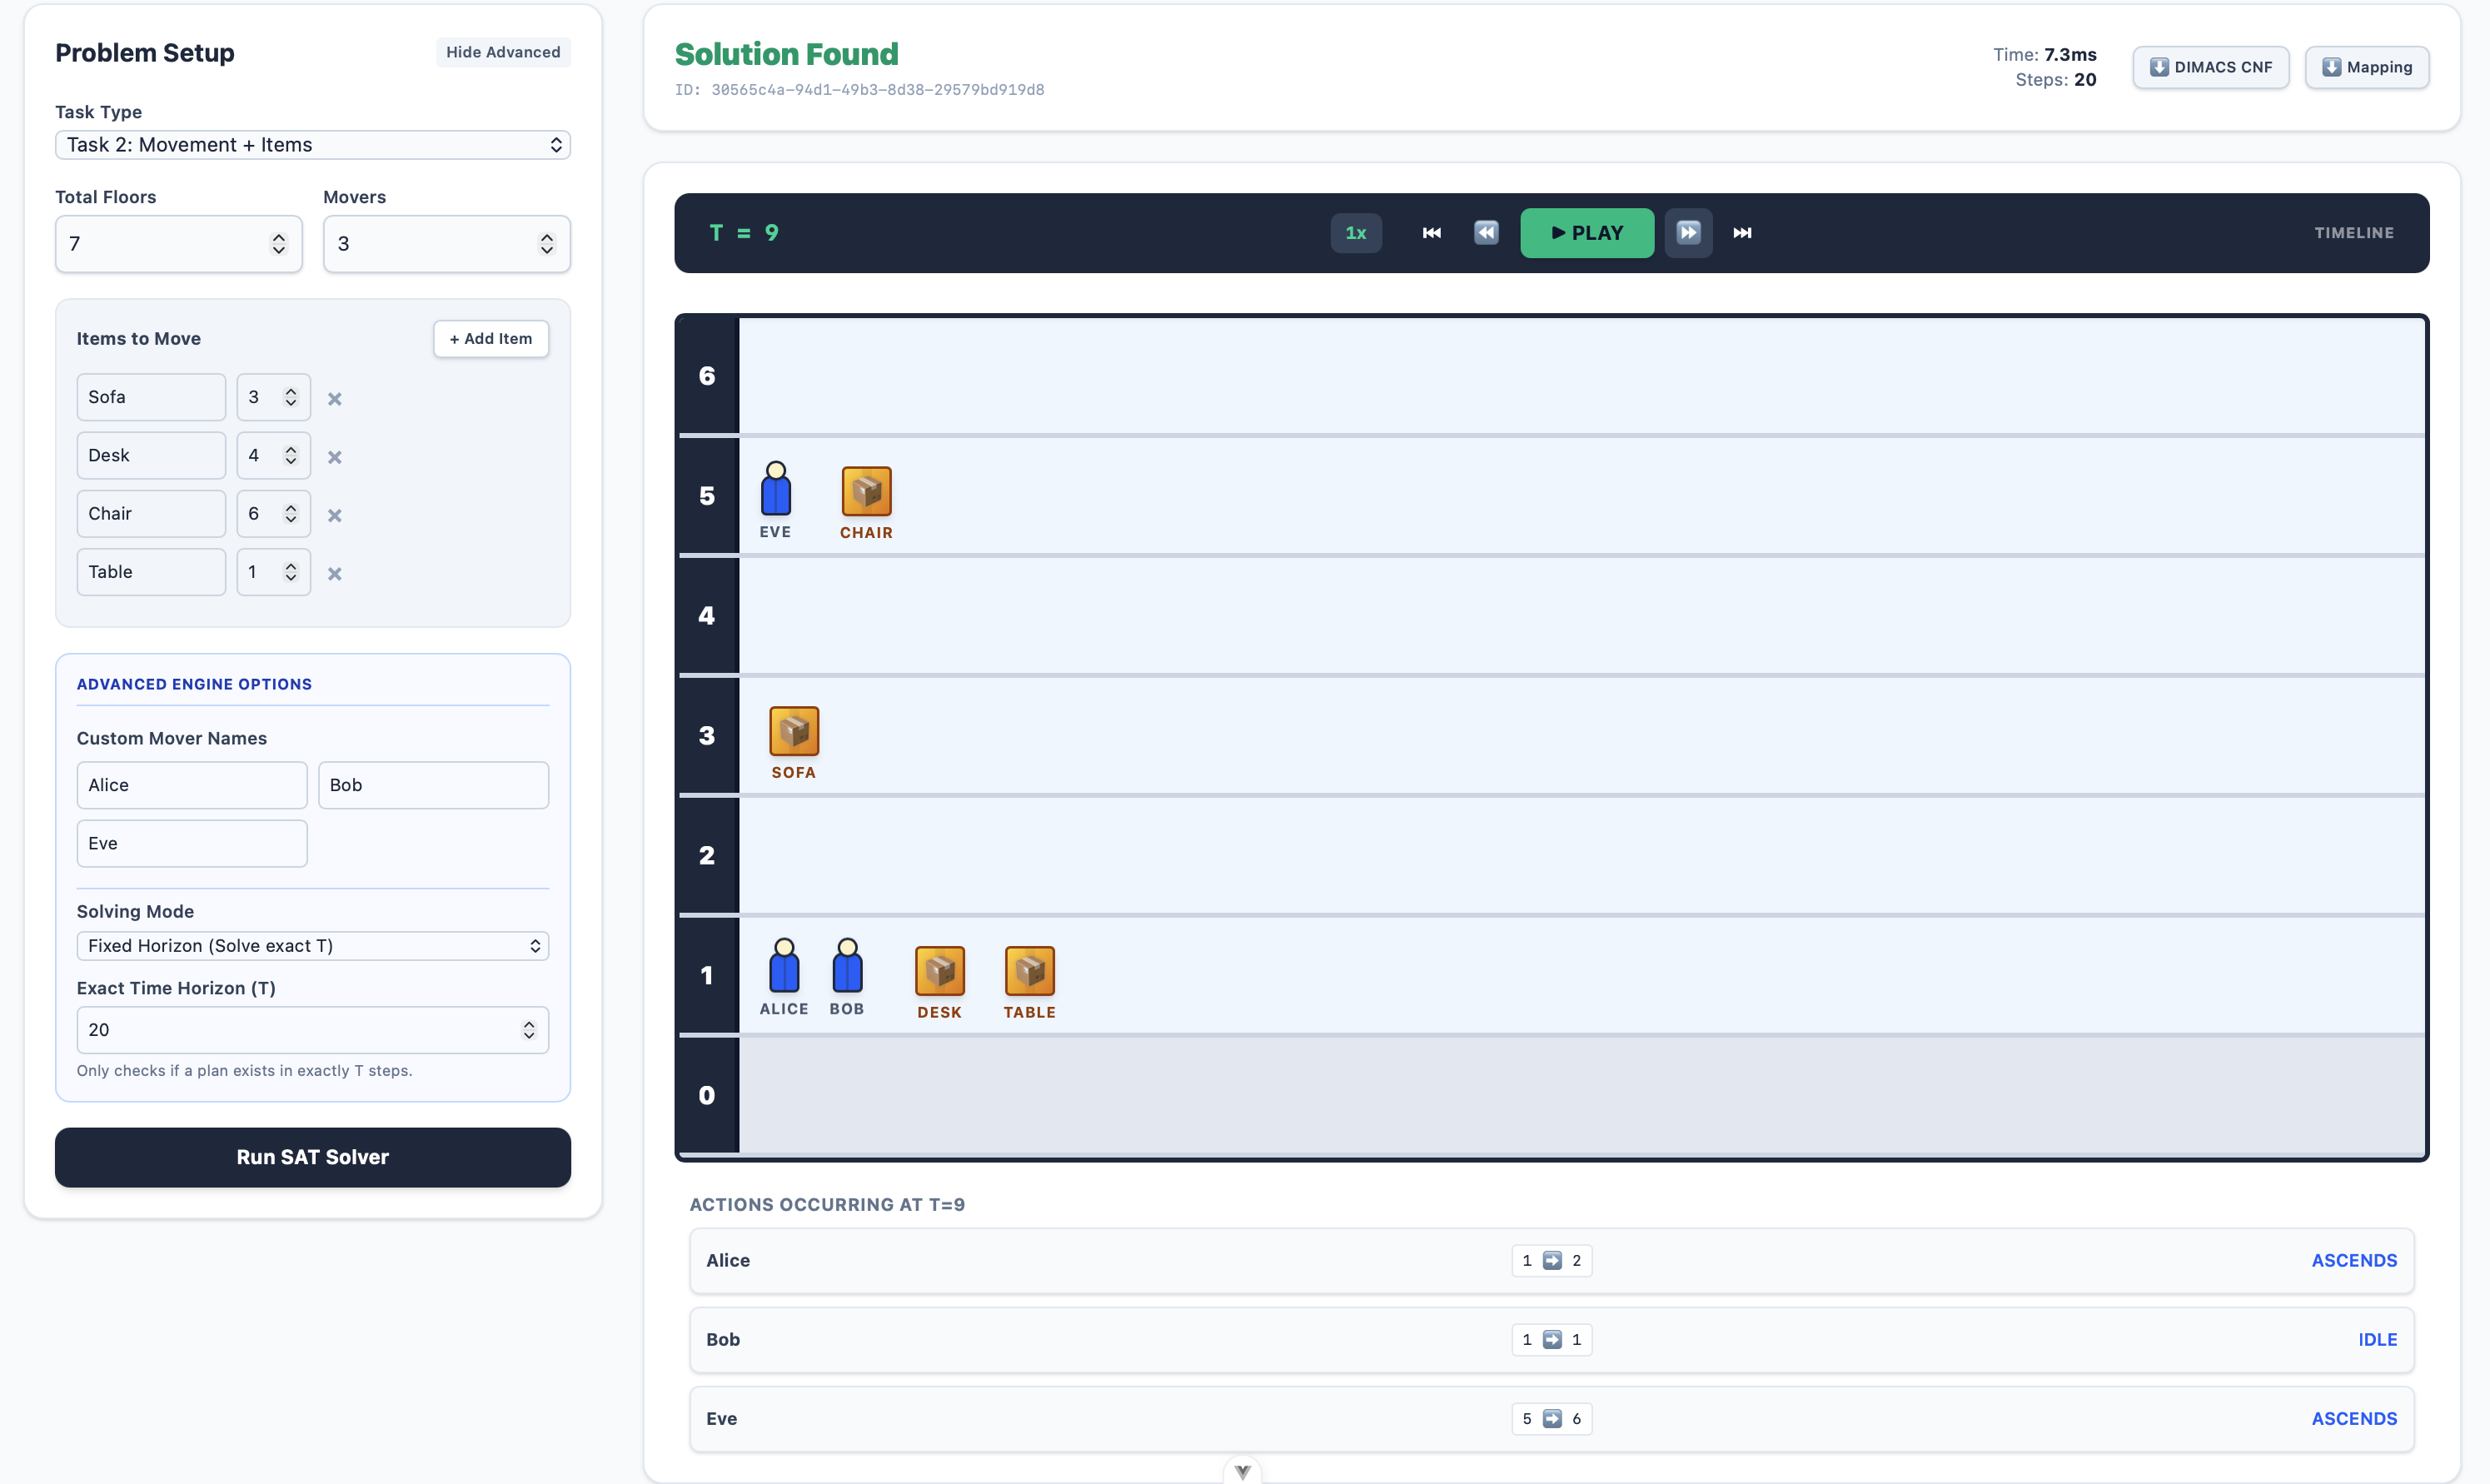
\includegraphics[width=0.95\textwidth]{img/task2-large-intermediate}
    \caption{Intermediate state of the larger instance, showing movers carrying items during the plan.}
    \label{fig:large-instance-middle}
\end{figure}

\begin{figure}[H]
    \centering
    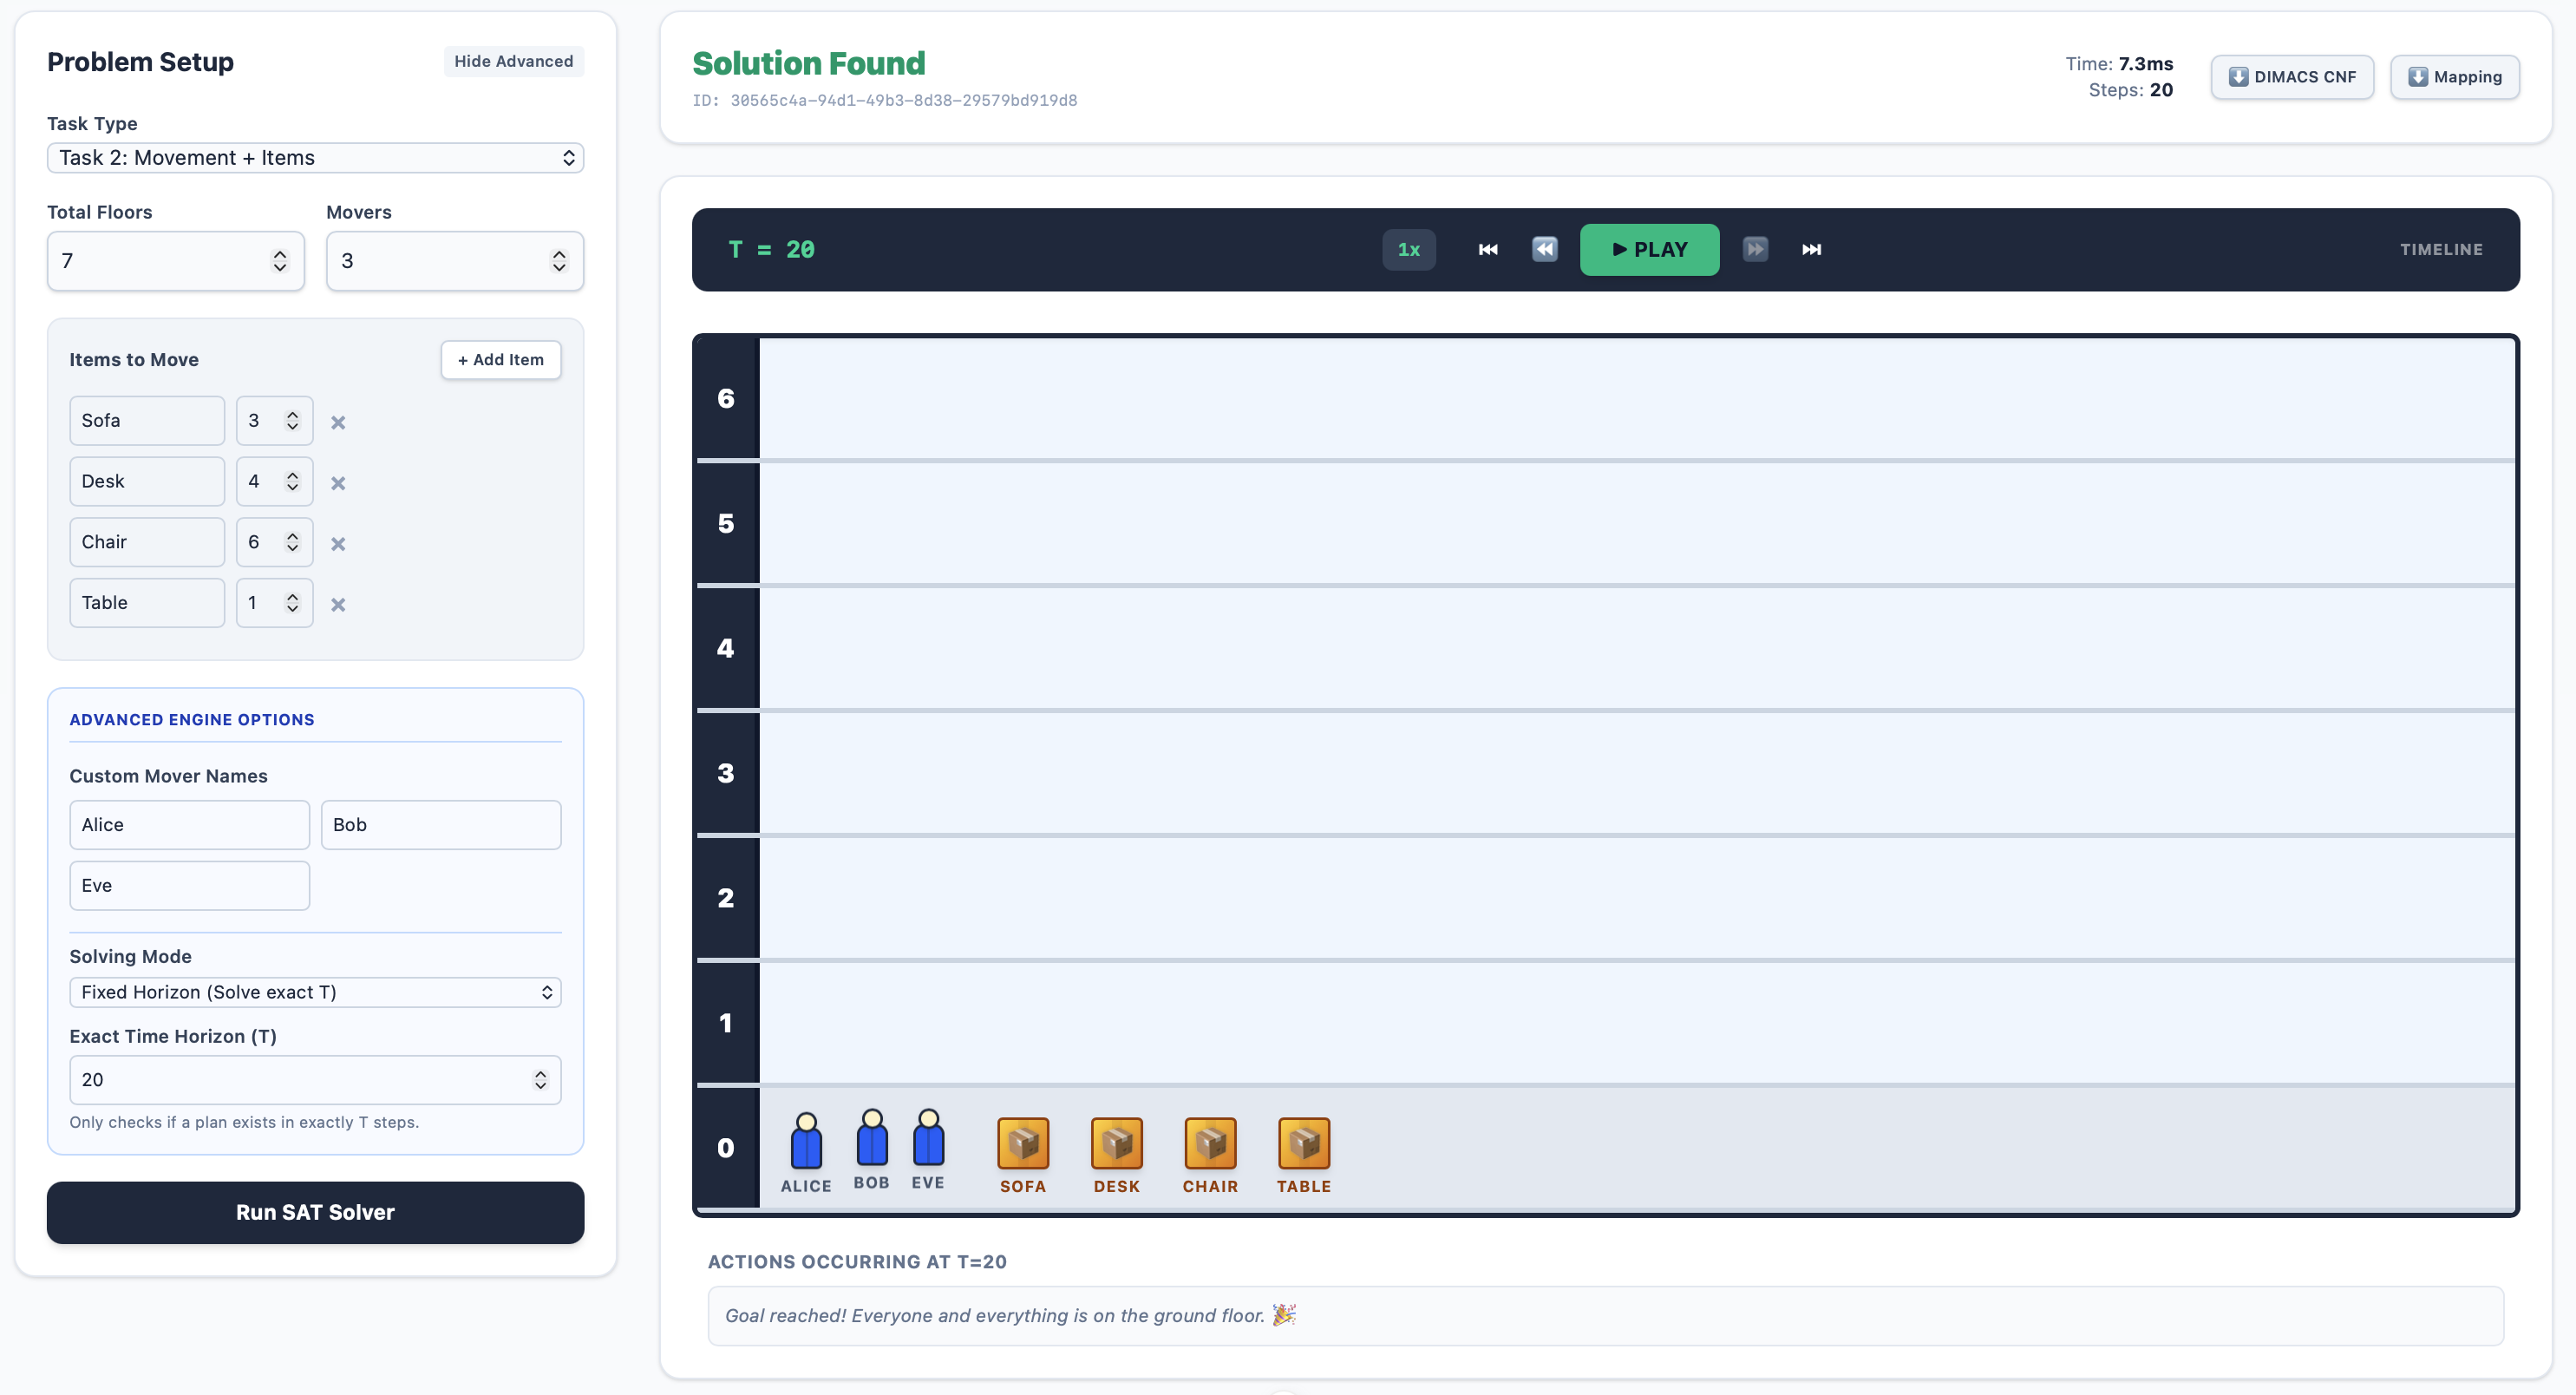
\includegraphics[width=0.95\textwidth]{img/task2-large-final}
    \caption{Final state of the larger instance, where all movers and items have reached the ground floor.}
    \label{fig:large-instance-final}
\end{figure}
    \newpage

    \section{Design Decisions and Issues} \label{sec:design-decisions-and-issues}

\subsection{General CNF Instead of 3-CNF} \label{subsec:general-cnf-instead-of-3-cnf}

The encoding uses general CNF clauses rather than forcing every clause to contain exactly three literals.
Although 3-SAT is important theoretically, converting every constraint into 3-CNF would require additional auxiliary variables and would make the implementation less readable.
General CNF is accepted directly by the PySAT solver interface, so this choice keeps the encoding simpler.

\subsection{Pairwise Cardinality Encoding} \label{subsec:pairwise-cardinality-encoding}

The system uses pairwise clauses for at-most-one constraints.
This produces $O(r^2)$ clauses for a group of $r$ literals, but the implementation is straightforward and works well for the tested problem sizes.

\subsection{Iterative Deepening for Optimality} \label{subsec:iterative-deepening-for-optimality}

Finding the shortest plan is achieved by repeatedly solving fixed-horizon instances.
This approach is easy to implement and gives a strong optimality guarantee: the first satisfiable horizon is the shortest possible one.

\subsection{Readable Mapping Output} \label{subsec:readable-mapping-output}

The project explicitly exports a mapping from integer SAT variables to readable names.
This is useful both for debugging and for satisfying the requirement that the SAT instance and truth assignment be interpretable.

\subsection{Frontend Visualization} \label{subsec:frontend-visualization}

The frontend is not required for the logical encoding itself, but it makes the solver much easier to understand.
Instead of only returning a list of Boolean assignments, the system shows a step-by-step animation of the plan.
    \newpage

    \section{Limitations} \label{sec:limitations}
The current implementation has some limitations:

\begin{itemize}
    \item Large instances can generate many clauses, especially due to pairwise at-most-one constraints.
    \item Iterative deepening may require solving many formulas before finding the optimal horizon.
    \item The in-memory cache used for retrieving CNF and mapping files does not persist after the backend restarts.
    \item The frontend is designed for moderate-sized examples; very large buildings or many movers/items may become visually crowded.
    \item The carrying model assumes that items only move down while carried.
    It does not model more complex actions such as passing items between people or carrying while staying on the same floor.
\end{itemize}
    \newpage

    \section{Conclusion} \label{sec:conclusion}
This project demonstrates how a logistics planning problem can be reduced to Boolean satisfiability.
By introducing variables for positions, actions, and carrying relations, the movement of movers and items through a building can be represented as a CNF formula.

\noindent The implementation supports both a movement-only version and a full movement-plus-items version of the problem.
The backend uses PySAT and Glucose3 to solve the generated formulas, while the frontend provides an interactive way to configure and visualize problem instances.

\noindent The solver successfully handles satisfiable and unsatisfiable cases, exports DIMACS CNF and variable mappings, and finds optimal plans using iterative deepening.
Overall, the project connects theoretical concepts from SAT and computational logic with a practical planning application.
    \newpage

    \begin{appendices}

        \section{User Guide} \label{sec:user-guide}

The project can be executed either with Docker Compose or manually by starting the backend and frontend separately.
The recommended method is Docker Compose, because it starts both services with a single command and avoids dependency conflicts.

\subsection{Docker Setup} \label{subsec:docker-setup}

The repository includes a \texttt{docker-compose.yml} file at the project root.
It defines two services:

\begin{itemize}
    \item \texttt{backend}: builds the FastAPI backend from \texttt{./backend} and exposes it on port \texttt{8000}.
    \item \texttt{frontend}: builds the Vue/Vite frontend from \texttt{./frontend} and exposes it on port \texttt{3000}.
\end{itemize}

\noindent To start the complete application using Docker, run the following command from the root directory of the project:

\begin{lstlisting}[language=bash,label={lst:start-docker}]
docker-compose up --build
\end{lstlisting}

\noindent After the containers are running, the application can be accessed at:

\begin{lstlisting}[language=bash, label={lst:endpoint-link}]
Frontend UI:      http://localhost:3000
Backend API docs: http://localhost:8000/docs
Backend API:      http://localhost:8000/api
\end{lstlisting}

\noindent To stop the application, press:

\begin{lstlisting}[language=bash, label={lst:stop-application}]
Ctrl+C
\end{lstlisting}

\noindent Alternatively, to stop and remove the containers, run:

\begin{lstlisting}[language=bash,label={lst:stop-docker}]
docker-compose down
\end{lstlisting}

\noindent The frontend container is configured with the environment variable:

\begin{lstlisting}[language=bash,label={lst:frontend-env}]
VITE_API_BASE_URL=http://localhost:8000/api
\end{lstlisting}

\noindent This means that, when the frontend is opened in the browser at \texttt{localhost:3000}, API requests are sent to the backend at \texttt{localhost:8000/api}.

\subsection{Backend Setup Without Docker} \label{subsec:backend-setup-without-docker}

To run the backend manually:

\begin{lstlisting}[language=bash,label={lst:run-backend}]
cd backend
python -m venv .venv
source .venv/bin/activate
pip install -r requirements.txt
uvicorn app.main:app --reload
\end{lstlisting}

\noindent On Windows, the virtual environment can be activated with:

\begin{lstlisting}[language=bash,label={lst:create-venv-window}]
.venv\Scripts\activate
\end{lstlisting}

\noindent The backend runs at:

\begin{lstlisting}[language=bash,label={lst:backend-link}]
http://localhost:8000
\end{lstlisting}

\noindent The API documentation is available at:

\begin{lstlisting}[language=bash,label={lst:api-doc-link}]
http://localhost:8000/docs
\end{lstlisting}

\subsection{Frontend Setup Without Docker} \label{subsec:frontend-setup-without-docker}

To run the frontend manually:

\begin{lstlisting}[language=bash, label={lst:run-frontend}]
cd frontend
npm install
npm run dev
\end{lstlisting}

\noindent When running through Docker, the frontend is available at:

\begin{lstlisting}[language=bash, label={lst:link-frontend-docker}]
http://localhost:3000
\end{lstlisting}

\subsection{CLI Examples} \label{subsec:cli-examples}

Task 1 example:

\begin{lstlisting}[language=bash,label={lst:example-1}]
python cli.py --floors 3 --persons 3 --task 1 --goal-floor 2
\end{lstlisting}

\noindent Task 2 example:

\begin{lstlisting}[language=bash,label={lst:example-2}]
python cli.py --floors 3 --persons 2 --items chair:1 table:2
\end{lstlisting}

\noindent Fixed-horizon solving:

\begin{lstlisting}[language=bash,label={lst:example-3}]
python cli.py --floors 3 --persons 2 --items chair:1 table:2 --fixed-t 5
\end{lstlisting}

\noindent Exporting DIMACS CNF:

\begin{lstlisting}[language=bash,label={lst:exporting-dimacs}]
python cli.py --floors 3 --persons 2 --items chair:1 table:2 --cnf-out problem.cnf
\end{lstlisting}
        \newpage

        \section{API Endpoints} \label{sec:api-endpoints}

\begin{table}[H]
    \centering
    \begin{tabular}{lll}
        \toprule
        \textbf{Method} & \textbf{Path}                       & \textbf{Description}                                \\
        \midrule
        POST            & \texttt{/api/solve}                 & Find the optimal solution using iterative deepening \\
        POST            & \texttt{/api/solve/fixed}           & Solve for an exact time horizon                     \\
        GET             & \texttt{/api/cnf/\{solve\_id\}}     & Retrieve the DIMACS CNF of a previous solve         \\
        GET             & \texttt{/api/mapping/\{solve\_id\}} & Retrieve the variable mapping of a previous solve   \\
        GET             & \texttt{/api/health}                & Health check endpoint                               \\
        \bottomrule
    \end{tabular}
    \caption{REST API endpoints exposed by the backend.}
    \label{tab:api-endpoints-table}
\end{table}

\newpage
        \newpage

        \section{Example API Request} \label{sec:example-api-request}

\begin{lstlisting}[language=bash,label={lst:example-api-request}]
curl -X POST http://localhost:8000/api/solve \
  -H "Content-Type: application/json" \
  -d `{
    "task": 2,
    "num_floors": 3,
    "num_persons": 2,
    "person_names": ["Alice", "Bob"],
    "items": [
      {"name": "Sofa", "initial_floor": 2},
      {"name": "Desk", "initial_floor": 1}
    ],
    "max_steps": 20
  }`
\end{lstlisting}
        \newpage

        \section{File Structure} \label{sec:file-structure}

\begin{lstlisting}[label={lst:folder-structure}]
TOC_MOVERS/
|-- docker-compose.yml
|-- README.md
|-- backend/
|   |-- Dockerfile
|   |-- README.md
|   |-- requirements.txt
|   |-- cli.py
|   |-- app/
|   |   |-- config.py
|   |   |-- main.py
|   |   |-- api/
|   |   |   |-- routes.py
|   |   |-- encoding/
|   |   |   |-- common_clauses.py
|   |   |   |-- task1_encoder.py
|   |   |   |-- task2_encoder.py
|   |   |   |-- variables.py
|   |   |-- models/
|   |   |   |-- problem.py
|   |   |-- output/
|   |   |   |-- dimacs.py
|   |   |   |-- mapping.py
|   |   |-- solver/
|   |       |-- decoder.py
|   |       |-- runner.py
|-- frontend/
|   |-- Dockerfile
|   |-- index.html
|   |-- public/
|   |-- src/
|       |-- main.js
|       |-- App.vue
|       |-- api/
|       |   |-- client.js
|       |-- assets/
|       |   |-- main.css
|       |-- components/
|           |-- ActionLog.vue
|           |-- BuildingVisualizer.vue
|           |-- ProblemSetup.vue
|           |-- ResultsPanel.vue
\end{lstlisting}
    \end{appendices}

\end{document}